\part{实例操作}

第四部分包含了CoLM2024发布版本的7个模拟实例。用户通过学习模拟实例的内容,一方面可以了解CoLM2024版本更完整的功能,另一方面,用户可以通过重现实验结果,迅速入门CoLM2024版本的使用。CoLM2024的模拟实例配置可以由define.h和namelist文件完全定义,第四部分内容将详细介绍每个实例的两个配置文件,并提供每个案例配置文件的可下载地址。结合本手册所提供的每个案例的重启文件、地表数据和气象驱动数据,每个模拟实例可以完全被重复。

\section{实例1:全球模拟}

本实例配置了一个常用的全球模拟的情景。实例使用了0.5\textdegree 的经纬度网格,植物群落(PC)方案的植被结构次网格,以及van Genuchten-Mualem土壤水特征曲线模型。该实例是CoLM2024版本的默认配置,模拟时间段为2005年1月1日到2005年12月31日。本实例关于配置文件、重启数据、地表数据和驱动数据的简介已罗列在表~\ref{ex1table}中。

\begin{table}[htbp]
\caption{实例1配置文件和数据一览表}
\centering \renewcommand{\arraystretch}{1.5}
\label{ex1table}
\begin{tabular}{llc}
\toprule
\textbf{数据名} & \textbf{文件/目录名} & \textbf{是否需要解压缩} \\\midrule

宏定义文件 & define.h & 否 \\
Namelist文件 & Global\_Grid\_50km\_PC\_VG.nml & 否 \\
地表数据 & landdata.tar.gz & 是 \\
气象驱动数据 & crujra2.5-2005.tar.gz & 是 \\
重启数据 & restart.tar.gz & 是 \\

\midrule

数据地址 & \multicolumn{2}{l}{大装置的地址}\\
\bottomrule
\end{tabular}
\end{table}


\subsection{实例1配置文件}\label{ex1config}

实例1的配置文件包含(1)\texttt{define.h}宏定义文件,控制模型大模块的开关,完整介绍见第三部分第~\ref{define.hux6587ux4ef6}节; (2)Namelist文件,控制模拟实例的具体信息,完整介绍见第三部分第~\ref{nml}节。

实例1的\texttt{define.h}文件内容为:
\lstinputlisting[language=fortran, basicstyle=\linespread{1.0}\footnotesize\ttfamily, commentstyle=\color{black}, numbers=left, numberstyle=\tiny, xleftmargin=1.5em,xrightmargin=0em, aboveskip=1em]{examples/global/define.h}

实例1的Namelist文件内容为,
\lstinputlisting[language=fortran, basicstyle=\linespread{1.0}\footnotesize\ttfamily, commentstyle=\color{black}, numbers=left, numberstyle=\tiny, xleftmargin=1.5em,xrightmargin=0em, aboveskip=1em]{examples/global/Global_Grid_50km_PC_VG.nml}

此实例中,\par
1)\textbf{并行化}方面,将全球分为20\textdegree$\times$20\textdegree 的数据块进行并行模拟(\texttt{DEF\_nx\_blocks=18}和\texttt{DEF\_ny\_blocks=9}),每54个进程为一个工作组(\texttt{DEF\_PIO\_groupsize=54});\par
2)\textbf{叶面积指数数据}使用了月变化数据(\texttt{DEF\_LAI\_MONTHLY=.true.}),且随年份变化(\texttt{DEF\_LAI\_CHANGE\_YEARLY=.true.});\par

3)对以下\textbf{过程参数化方案}进行了设置:
\begin{itemize}[nosep,leftmargin=4em]
    \item 降水截留(\texttt{DEF\_Interception\_scheme=1});
    \item 土壤阻抗(\texttt{DEF\_RSS\_SCHEME=1});
    \item 土壤水运动数值方案(\texttt{DEF\_USE\_VariablySaturatedFlow=.true.});
    \item 过冷水方案(\texttt{DEF\_USE\_SUPERCOOL\_WATER=.true.});
    \item 产流参数化方案(\texttt{DEF\_Runoff\_SCHEME=3});
    \item 植被水力过程方案(\texttt{DEF\_USE\_PLANTHYDRAULICS=.true.});
    \item 水利用效率最优气孔方案(\texttt{DEF\_USE\_WUEST=.true.});
    \item 植物群落次网格简化方案(\texttt{DEF\_FAST\_PC=.true.});

\end{itemize}
\par
4)模型模拟的起始时间为2005年1月1日,模拟的结束时间为2005年12月31日\par

5)模型模拟采用0.5 \textdegree $\times$ 0.5 \textdegree 的经纬度网格\par

6)使用CRUJRA数据作为\textbf{大气驱动}(\texttt{DEF\_forcing\_namelist=<path>/CRUJRA.nml});\par
7)每年保存一次\textbf{重启动}文件(\texttt{DEF\_WRST\_FREQ=‘YEARLY’});\par
8)\textbf{历史数据的输出},
\begin{itemize}[nosep,leftmargin=4em]
    \item 输出到0.5\textdegree 经纬度网格(\texttt{DEF\_hist\_lon\_res=0.5}和\texttt{DEF\_hist\_lon\_res=0.5});
    \item 输出变量的月值(\texttt{DEF\_HIST\_FREQ='MONTHLY'});
    \item 每月的数据保存在一个文件中(\texttt{DEF\_HIST\_groupby='MONTH'});
    \item 输出所有变量(\texttt{DEF\_hist\_vars\_out\_default=.true.}).
\end{itemize}\par
9)其他配置使用模式默认值。

\subsection{实例1地表数据}

地表数据的制作由CoLM2024版本地表制作程序(mksrfdata.x)基于~\ref{ex1config}节介绍的配置文件制作而成。实例1的地表数据制作基于全球经纬度网格,为了提高并行效率,地表制作程序将全球区域分为经向18个$\times$纬向9个网格。地表制作程序按植物群落次网格的方式划分模拟计算单元,从土壤属性和地表覆盖等高分辨率基础数据集出发,计算并聚合得出每个计算单元的土壤水力参数、热力参数、叶面积指数、植被功能型覆盖比例、湖深、树高、地形和土壤质地等模型运行所需的重要参数或变量。

\subsection{实例1气象驱动数据}\label{ex1forcing}

实例1使用Climate Research Unit and Japanese Reanalysis(CRUJRA)气象驱动数据,整合了来自英国气候研究组和日本再分析项目的优质资源。本实例使用CRUJRA 2005年的数据驱动模型。使用CRUJRA驱动需要在Namelist文件中设置CRUJRA Namelist文件的地址,见~\ref{ex1config}。CRUJRA Namelist文件(CRUJRA.nml)可以在代码根目录中的run/forcing/子目录下找到。CRUJRA Namelist文件存储了CRUJRA的格式信息和驱动地址。在新机器配置时,需要重新设置CRUJRA存储地址(\texttt{DEF\_dir\_forcing=/path/to/crujra/})。

\subsection{实例1重启数据}

重启数据存储了模型运行中的状态变量,重启数据可以由冷启动生成或前序模拟生成。实例1的模拟初始于2005年1月1日,其重启数据由前序模拟生成。前序模拟的方案配置与~\ref{ex1config}节内容基本相同,模拟时间从1996年1月1日开始到2004年12月31日结束,重启文件每年存储一次,模拟结束时所生成的重启文件被用于实例1的模拟初始化。

\subsection{实例1操作步骤}

\textbf{第1步}:修改宏定义文件\texttt{define.h}

该文件位于源代码\texttt{include}目录下,可根据章节~\ref{ex1config} 进行修改,或者用本指南提供的宏定义文件进行覆盖。

\bigskip
\textbf{第2步}:建立实例运行Namelist文件

在任意目录下建立用于实例运行的Namelist文件,可参考章节~\ref{ex1config} Namelist文件部分进行修改或者用本指南所提供的文件\texttt{Global\_Grid\_50km\_PC\_VG.nml}覆盖。

\bigskip
\textbf{第3步}:建立实例目录

用户新建实例目录,目录命名与Namelist文件的\texttt{DEF\_CASE\_NAME}设置保持一致(本例中即Global\_Grid\_50km\_PC\_VG)。本实例已提供地表数据,因此用户需手动建立实例目录。另外,需修改Namelist文件中的\texttt{DEF\_dir\_output}值为实例文件夹所在的目录(即父目录),比如:实例目录的路径是/path/to/Global\_Grid\_50km\_PC\_VG,\texttt{DEF\_dir\_output}须设置为/path/to/。

\bigskip
\textbf{第4步}:准备地表数据

解压指南所提供的本实例地表数据文件\texttt{landdata.tar.gz},解压后得到的文件夹\texttt{landdata}放置于实例目录下。

\bigskip
\textbf{第5步}:准备驱动数据

解压指南所提供的本实例驱动文件\texttt{crujra2.5-2005.tar.gz },修改解压后的驱动配置文件\texttt{CRUJRA.nml}:通过修改变量\texttt{DEF\_dir\_forcing}设置,指定驱动路径。最后,须确保Namelist文件中的\texttt{DEF\_forcing\_namelist}设置与驱动配置文件\texttt{CRUJRA.nml}的路径一致。

\bigskip
\textbf{第6步}:编译源代码

进入到源代码主目录,运行\texttt{make}命令进行编译,
\begin{quote}
\begin{lstlisting}
make
\end{lstlisting}
\end{quote}

\bigskip
\textbf{第7步}:运行初始化程序

本实例为用户提供了重启数据,可以依赖重启数据进行热启动。解压指南所提供的本实例重启数据文件\texttt{restart.tar.gz},解压后得到的文件夹\texttt{restart}放置于实例目录下。

\bigskip
\textbf{第8步}:执行主程序

在\texttt{run}目录下,执行
\begin{quote}
\begin{lstlisting}
mpirun -np $nproc ./colm.x Global_Grid_50km_PC_VG.nml
\end{lstlisting}
\end{quote}

其中,\$nproc为实际使用的计算核心数。成功执行后,模式运行结果会在实例目录下的history文件夹中输出。


\subsection{实例1的模拟结果展示}

实例1中,CoLM2024的发布版本实现了2005年的全球0.5度分辨率模拟,其中年均潜热全球空间分布模拟结果见图~\ref{fig:fig_example01_qle}。CoLM2024模型对2005年全球年平均潜热通量(Qle)的模拟结果展现出高度的物理合理性,其分布特征与观测数据相吻合。模拟成功地再现了赤道及低纬度地区(如亚马逊雨林、东南亚)因强对流和植被蒸散作用形成的高潜热通量(>120 W/m²),以及副热带干旱区(如撒哈拉沙漠)受水分限制导致的低值带(<40 W/m²)。模拟结果合理呈现了中高纬度陆地(如西伯利亚)因低温冰雪覆盖导致的潜热抑制现象,并与南半球海洋主导的活跃潜热释放(60-100 W/m²)形成对比,体现了海陆热力差异的物理响应。模型未出现与气候背景矛盾的异常值,空间梯度过渡自然,基本展示出陆气水热交换特征。

\begin{figure}[htpb]
    \centering
    \includegraphics[width=0.90\textwidth]{figures/Example01_Qle_Global_Grid_50km_PC_VG.jpg}
    \caption{CoLM2024模拟结果(2005年):潜热年平均($\mathrm{W \cdot m^{-2}}$)全球分布}
    \label{fig:fig_example01_qle}
\end{figure}

\section{实例2:自然植被下垫面单点模拟}

\subsection{实例2配置文件}\label{ex2config}

本节配置了一个使用自然地表数据集运行的单点模拟实例。实例使用植物群落(PC)植被结构次网格,以及van Genuchten-Mualem土壤水特征曲线模型,实时输出调试信息。在单点模式下,自动关闭并行功能。本实例关于配置文件、重启数据、地表数据和驱动数据的简介已列于表~\ref{ex2table} 中。


\begin{table}[htbp]
\caption{实例2配置文件和数据一览表}
\centering \renewcommand{\arraystretch}{1.5}
\label{ex2table}
\begin{tabular}{llc}
\toprule
\textbf{数据名} & \textbf{文件/目录名} & \textbf{是否需要解压缩} \\

\midrule

宏定义文件 & define.h & 否 \\
Namelist文件 & Site\_IT-Isp.nml & 否 \\
地表数据 & srfdata.nc & 否 \\
气象驱动数据及\\Namelist文件 & IT-Isp\_2013-2014\_FLUXNET2015\_Met.tar.gz & 是 \\
%重启数据 & restart.tar.gz & 是 \\

\bottomrule
\end{tabular}
\end{table}

\texttt{define.h}文件的内容为,
\lstinputlisting[language=fortran, basicstyle=\linespread{1.0}\footnotesize\ttfamily, commentstyle=\color{black}, numbers=left, numberstyle=\tiny, xleftmargin=1.5em,xrightmargin=0em, aboveskip=1em]{examples/site_nature/define.h}

Namelist文件的内容为,
\lstinputlisting[language=fortran, basicstyle=\linespread{1.0}\footnotesize\ttfamily, commentstyle=\color{black}, numbers=left, numberstyle=\tiny, xleftmargin=1.5em,xrightmargin=0em, aboveskip=1em]{examples/site_nature/Site_IT-Isp.nml}

此实例中,\par
1)模拟点的地表覆盖类型、植被功能型组成及占比、树高、叶面积指数和土壤水热参数从站点数据\texttt{\$SITE\_fsitedata}读取,土壤反照率、地形参数根据站点经纬度(\texttt{SITE\_lon\_location}和\texttt{SITE\_lat\_location})\textbf{从CoLM自带的全球地表数据集中提取};\par
2)模拟时间为2013年至2014年,其中2013年为预热,预热阶段重复两次;\par
3)使用了逐年变化(\texttt{DEF\_LAI\_CHANGE\_YEARLY})\textbf{叶面积指数月数据}\\ (\texttt{DEF\_LAI\_MONTHLY});\par
4)土壤阻抗方案选择Seller等人1992年方案(\texttt{DEF\_RSS\_SCHEME});\par
5)使用模拟点观测的的\textbf{大气驱动数据}(通过\texttt{DEF\_forcing\_namelist}设置);\par
6)每月保存一次\textbf{重启动}变量(\texttt{DEF\_WRST\_FREQ});\par
7)\textbf{历史数据的输出},
\begin{itemize}[nosep,leftmargin=4em]
    \item 输出变量为每步长值(\texttt{DEF\_HIST\_FREQ});
    \item 每年的数据保存在一个文件中(\texttt{DEF\_HIST\_groupby});
    \item 不对重启动文件进行压缩(\texttt{DEF\_HIST\_CompressLevel})
    \item 输出所有变量(\texttt{DEF\_hist\_vars\_out\_default}).
\end{itemize} \par
8)其余配置使用模式默认值。

\subsection{实例2地表数据}

实例2基于单点模拟,模拟一个自然地表站点的陆面过程。其地表数据部分来源于站点观测,部分来源于全球数据,根据Namelist设置读取。使用的站点观测参数有地表覆盖类型、植被功能型组成及占比、树高、叶面积指数和土壤水热参数。除以上数据外,土壤反照率等数据根据站点经纬度从全球数据提取。

\subsection{实例2操作步骤}

\textbf{第1步}:修改宏定义文件\texttt{define.h}

该文件位于源代码\texttt{include}目录下,可根据章节~\ref{ex2config} 进行修改,或者本指南提供的相应文件覆盖。

\bigskip
\textbf{第2步}:建立实例运行Namelist文件

在源代码\texttt{run}目录下建立用于实例运行Namelist文件,可参考章节~\ref{ex2config} Namelist文件部分或者本指南提供的文件\texttt{Site\_IT-Isp.nml}覆盖。

\bigskip
\textbf{第3步}:建立实例目录

用户新建实例目录文件夹,命名与\texttt{Site\_IT-Isp.nml}的\texttt{DEF\_CASE\_NAME}设置保持一致。如用户自己制作地表数据,该目录会根据\texttt{DEF\_CASE\_NAME}自动创建。本实例已提供地表数据,因此用户需手动建立实例目录。另外,需修改\texttt{Site\_IT-Isp.nml}中的\texttt{DEF\_dir\_output}值为实例文件夹所在的目录(即父目录)。

\bigskip
\textbf{第4步}:准备地表数据

将指南所提供的本实例地表数据文件\texttt{srfdata.nc}放置于实例目录\texttt{landdata}下。

\bigskip
\textbf{第5步}:准备驱动数据

解压指南所提供的本实例驱动文件\texttt{IT-Isp\_2013-2014\_FLUXNET2015\_Met.tar.gz},修改解压后的驱动配置文件\texttt{IT-Isp.nml},通过变量\texttt{DEF\_dir\_forcing}设置解压得到的驱动文件\texttt{IT-Isp\_2013-2014\_FLUXNET2015\_Met.nc}所在的路径。

修改实例Namelist文件驱动配置文件路径\texttt{DEF\_forcing\_namelist}。

\bigskip
\textbf{第6步}:编译源代码

进入到源代码主目录,运行\texttt{make}命令进行编译,
\begin{quote}
\begin{lstlisting}
make
\end{lstlisting}
\end{quote}

\bigskip
\textbf{第7步}:运行初始化程序

进入到源代码下\texttt{run}目录,运行
\begin{quote}
\begin{lstlisting}
./mkinidata.x Site_IT-Isp.nml
\end{lstlisting}
\end{quote}

成功执行后,初始化数据会在实例目录下的restart文件夹中生成。

\bigskip
\textbf{第8步}:执行主程序

在\texttt{run}目录下,执行
\begin{quote}
\begin{lstlisting}
./colm.x Site_IT-Isp.nml
\end{lstlisting}
\end{quote}

成功执行后,模式运行结果会在实例目录下的history文件夹中输出。

\subsection{实例2模拟结果展示}

本实例模型输出结果文件为\texttt{IT-Isp\_hist\_2014.nc},下图为模式模拟的2014年日平均潜热通量(在文件中的变量名为\texttt{f\_lfevpa})时间序列图,同时与通量塔观测数据的对比。观测数据可通过提供的参考数据文件\texttt{IT-Isp\_2013-2014\_FLUXNET2015\_Flux.nc}中变量\texttt{Qle\_cor}得到。

\begin{figure}[htpb]
    \centering
    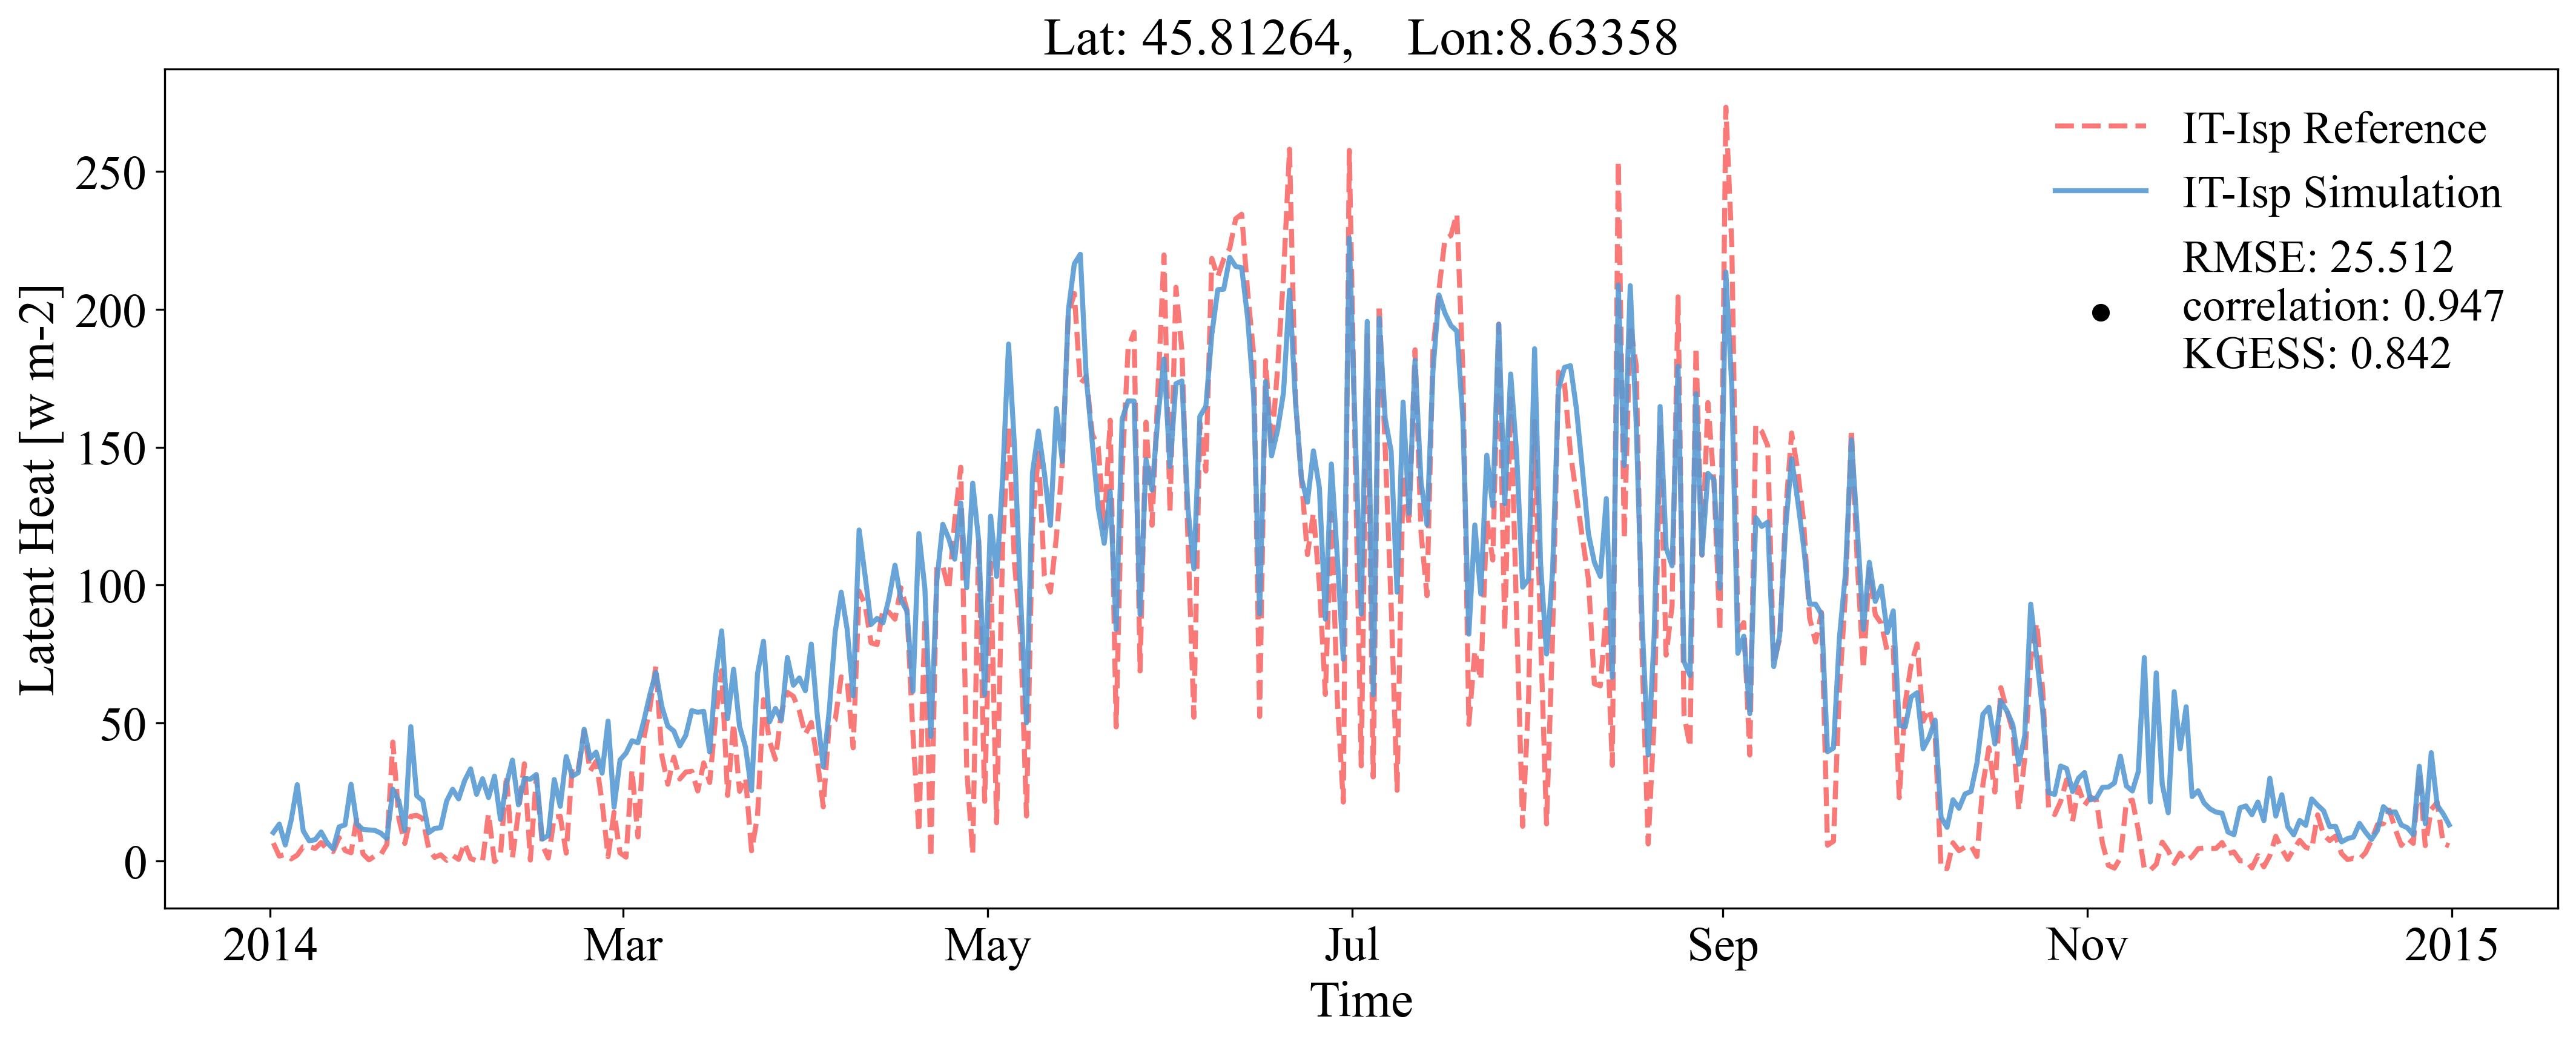
\includegraphics[width=0.90\textwidth]{figures/Example02_Site_IT-Isp.jpg}
    \caption{CoLM2024模拟IT-Isp站点潜热通量日均值及与观测对比结果(单位:\unit{W.m^{-2}})}
    \label{fig:fig_example02_IT}
\end{figure}

\section{实例3:城市单点模拟}

本实例配置了一个用于国际城市模式比较计划的城市单点模拟。实例的地表覆盖类型为城市,打开了CoLM 2024版新城市模块,使用Campbell土壤水特征曲线模型,实时输出调试信息及检查变量范围。在单点模式下,自动关闭并行功能。本实例关于配置文件、重启数据、地表数据和驱动数据的简介已罗列在表~\ref{ex3table} 中。


\begin{table}[htbp]
\caption{实例3配置文件和数据一览表}
\centering \renewcommand{\arraystretch}{1.5}
\label{ex3table}
\begin{tabular}{llc}
\toprule
\textbf{数据名} & \textbf{文件/目录名} & \textbf{是否需要解压缩} \\

\midrule

宏定义文件 & define.h & 否 \\
Namelist文件 & Site\_AU-Preston.nml & 否 \\
地表数据 & srfdata.nc & 否 \\
气象驱动数据及\\Namelist文件 & AU-Preston\_metforcing\_v1.tar.gz & 是 \\
% 重启数据 & restart.tar.gz & 是 \\

\bottomrule
\end{tabular}
\end{table}

\subsection{实例3配置文件}\label{ex3config}
实例3的配置文件包含(1) \texttt{define.h}宏定义文件,控制模型大模块的开关,本实例的SinglePoint、URBAN\_MODEL以及Campbell\_SOIL\_MODEL土壤水特征曲线模型开关通过宏定义文件控制; (2)Namelist文件,控制模拟实例的具体信息,本实例的Namelist文件的主要配置为:a) 使用站点观测的建筑形态、生态、辐射以及人类活动数据;b) 开启叶面积指数年际变化;c) 使用LCZ分类模拟城市;d) 开启城市植被、水体、人为热模拟;e) 使用CoLM2014叶片截流方案;f) spin-up结束后按时间步长输出模拟结果。

\texttt{define.h}文件的内容为:
\lstinputlisting[language=fortran, basicstyle=\linespread{1.0}\footnotesize\ttfamily, commentstyle=\color{black}, numbers=left, numberstyle=\tiny, xleftmargin=1.5em,xrightmargin=0em, aboveskip=1em]{examples/site_urban/define.h}

Namelist文件的内容为:
\lstinputlisting[language=fortran, basicstyle=\linespread{1.0}\footnotesize\ttfamily, commentstyle=\color{black}, numbers=left, numberstyle=\tiny, xleftmargin=1.5em,xrightmargin=0em, aboveskip=1em]{examples/site_urban/Site_AU-Preston.nml}

此实例中,\par
1)模拟站点的土壤水热参数、湖泊深度、建筑热属性参数、除屋顶反照率外的其它辐射参数、人为热模块等属性参数根据模拟点的经纬度(从\texttt{\$SITE\_fsitedata}中读取)\textbf{从CoLM自带的地表数据集中提取或者根据建筑类型赋值};\par
2)模拟站点的建筑几何形态(建筑高度、比例等)、生态(树覆盖度、树高、湖泊覆盖度等)、辐射(屋顶反照率)、人类活动(人口密度)等城市参数来源于数据文件\texttt{\$SITE\_fsitedata};\par
3)模拟时间为1993年至2004年,其中2003年8月12日前为预热;\par
4)对以下\textbf{城市参数化方案}进行了设置:
\begin{itemize}[nosep,leftmargin=4em]
    \item 使用LCZ城市分类(\texttt{DEF\_URBAN\_type\_scheme=2});
    \item 模拟城市中的植被(\texttt{DEF\_URBAN\_TREE=.true.});
    \item 模拟城市中的水体(\texttt{DEF\_URBAN\_WATER=.true.});
    \item 模拟城市中的建筑能耗排放(\texttt{DEF\_URBAN\_BEM=.true.});
    \item 模拟城市中的交通热以及人体代谢热(\texttt{DEF\_URBAN\_LUCY=.true.});
    \item 使用三维建筑高边长比参数(\texttt{DEF\_USE\_CANYON\_HWR=.false.});
\end{itemize} \par
5)使用了逐年变化(\texttt{DEF\_LAI\_CHANGE\_YEARLY})\textbf{叶面积指数月数据};\par
6)对以下\textbf{过程参数化方案}进行了设置:
\begin{itemize}[nosep,leftmargin=4em]
    \item 使用CoLM2014降水截留方案(\texttt{DEF\_Interception\_scheme=1});
    \item 不使用过冷水方案(\texttt{DEF\_USE\_SUPERCOOL\_WATER=.false.});
    \item 不使用变饱和土壤水运动算法(\texttt{DEF\_USE\_VariablySaturatedFlow=.false.});
    \item 不使用植被水力过程方案(\texttt{DEF\_USE\_PLANTHYDRAULICS=.false.});
    \item 不使用水利用效率最优气孔方案(\texttt{DEF\_USE\_WUEST=.false.});
    \item 不使用SNICAR模块(\texttt{DEF\_USE\_SNICAR=.false.});
    \item 未将土壤和积雪表面的热力过程分开计算(\texttt{DEF\_SPLIT\_SOILSNOW=.false.});
    \item 不使用植被积雪模块(\texttt{DEF\_VEG\_SNOW=.false.});
\end{itemize}
\par
7)使用模拟点观测的的\textbf{大气驱动数据}(通过\texttt{DEF\_forcing\_namelist=<path>/AU-Preston.nml}设置);\par
8)每月保存一次\textbf{重启动}变量(\texttt{DEF\_WRST\_FREQ='MONTHLY'}),不对重启动文件进行压缩(\texttt{DEF\_\allowbreak REST\_\allowbreak CompressLevel=0});\par
9)\textbf{历史数据的输出},
\begin{itemize}[nosep,leftmargin=4em]
    \item 输出每个步长的变量值(\texttt{DEF\_HIST\_FREQ='TIMESTEP'});
    \item 每月的数据保存在一个文件中(\texttt{DEF\_HIST\_groupby='MONTH'});
    \item 不对重启动文件进行压缩(\texttt{DEF\_HIST\_CompressLevel=0})
    \item 输出所有变量(\texttt{DEF\_hist\_vars\_out\_default=.true.}).
\end{itemize} \par
10)其余配置使用模式默认值。

\subsection{实例3地表数据}

实例3基于单点模拟,模拟一个城市站点的陆面过程。其地表数据部分来源于站点观测,部分来源于全球原始数据。其中,根据Namelist设置,使用的站点观测参数如表~\ref{ex3table_para} 所示。

\begin{table}[htbp]
\caption{站点观测参数}
\centering \renewcommand{\arraystretch}{1.5}
\label{ex3table_para}
\begin{tabular}{llc}
\toprule
\textbf{Namelist配置} & \textbf{数据类型} & \textbf{数据名称} \\

\midrule

\texttt{USE\_SITE\_urban\_geometry} & 建筑形态 & 建筑高度、建筑比例、三维建筑高边长比  \\
\texttt{USE\_SITE\_urban\_ecology} & 城市生态 & 树覆盖度、树高、湖泊覆盖度 \\
\texttt{USE\_SITE\_urban\_radiation} & 辐射属性 & 屋顶反照率  \\
\texttt{USE\_SITE\_urban\_human} & 人类活动 & 人口密度  \\

\bottomrule
\end{tabular}
\end{table}

除表中数据外,土壤反照率、土壤水热参数、湖泊深度、城市树LAI/SAI、建筑热属性以及BEM/LUCY人为热模块需要的参数均根据站点经纬度从全球数据提取或根据建筑类型赋值。

\subsection{实例3操作步骤}

\textbf{第1步}:修改宏定义文件\texttt{define.h}

该文件位于源代码\texttt{include}目录下,可根据章节~\ref{ex3config} 进行修改,或者本指南提供的相应文件覆盖。

\bigskip
\textbf{第2步}:建立实例运行Namelist文件

在源代码\texttt{run}目录下建立用于实例运行Namelist文件,可参考章节~\ref{ex3config} Namelist文件部分或者本指南提供的文件\texttt{Site\_AU-Preston.nml}覆盖。

\bigskip
\textbf{第3步}:建立实例目录

用户新建实例目录文件夹,命名与\texttt{Site\_AU-Preston.nml}的\texttt{DEF\_CASE\_NAME}设置保持一致。如用户自己制作地表数据,该目录会根据\texttt{DEF\_CASE\_NAME}自动创建。本实例已提供地表数据,因此用户需手动建立实例目录。另外,需修改\texttt{Site\_AU-Preston.nml}中的\texttt{DEF\_dir\_output}值为实例文件夹所在的目录(即父目录)。

\bigskip
\textbf{第4步}:准备地表数据

将指南所提供的本实例地表数据文件\texttt{srfdata.nc}放置于实例目录\texttt{landdata}下。

\bigskip
\textbf{第5步}:准备驱动数据

解压指南所提供的本实例驱动文件\texttt{AU-Preston\_metforcing\_v1.tar.gz},修改解压后的驱动配置文件\texttt{AU-Preston.nml},通过变量\texttt{DEF\_dir\_forcing}设置解压得到的驱动文件\texttt{AU-Preston\_metforcing\_v1.nc}所在的路径。

修改实例Namelist文件驱动配置文件路径\texttt{DEF\_forcing\_namelist}。

\bigskip
\textbf{第6步}:编译源代码

进入到源代码主目录,运行\texttt{make}命令进行编译,
\begin{quote}
\begin{lstlisting}
make
\end{lstlisting}
\end{quote}

\bigskip
\textbf{第7步}:运行初始化程序

进入到源代码下\texttt{run}目录,运行
\begin{quote}
\begin{lstlisting}
./mkinidata.x Site_AU-Preston.nml
\end{lstlisting}
\end{quote}

成功执行后,初始化数据会在实例目录下的restart文件夹中生成。

\bigskip
\textbf{第8步}:执行主程序

在\texttt{run}目录下,执行
\begin{quote}
\begin{lstlisting}
./colm.x Site_AU-Preston.nml
\end{lstlisting}
\end{quote}

成功执行后,模式运行结果会在实例目录下的history文件夹中输出。

% \subsection{实例3重启数据}

% 实例3的模拟初始于2003年8月12日,其重启数据由前序模拟生成。前序模拟的方案配置与章节~\ref{ex3config} 相同,模拟时间从1992年12月31日开始到2003年8月12日结束,由于该阶段重启文件每年存储一次,因此用户可使用2003年1月1日的重启文件用于实例3的初始化。

\subsection{实例3模拟结果展示}

实例3中,CoLM2024的发布版本实现了城市单点模拟,其日变化模拟结果见图~\ref{fig:fig_example03_au}。CoLM2024城市模型对AU-Preston的模拟结果与观测相比十分吻合。模拟成功地再现了该站点的辐射以及湍流通量平均日变化,而且与观测相比,短波与长波的RMSE分别为3.63W/m²和6.42W/m²,净辐射RMSE同样仅有7.65W/m²,而感热通量与潜热通量的RMSE分别为35.08W/m²以及37.79W/m²,而对于储热通量,其RMSE为48.03W/m²,对于时间步长(30分钟)的验证而言模拟结果已经较为准确。

\begin{figure}[htpb]
    \centering
    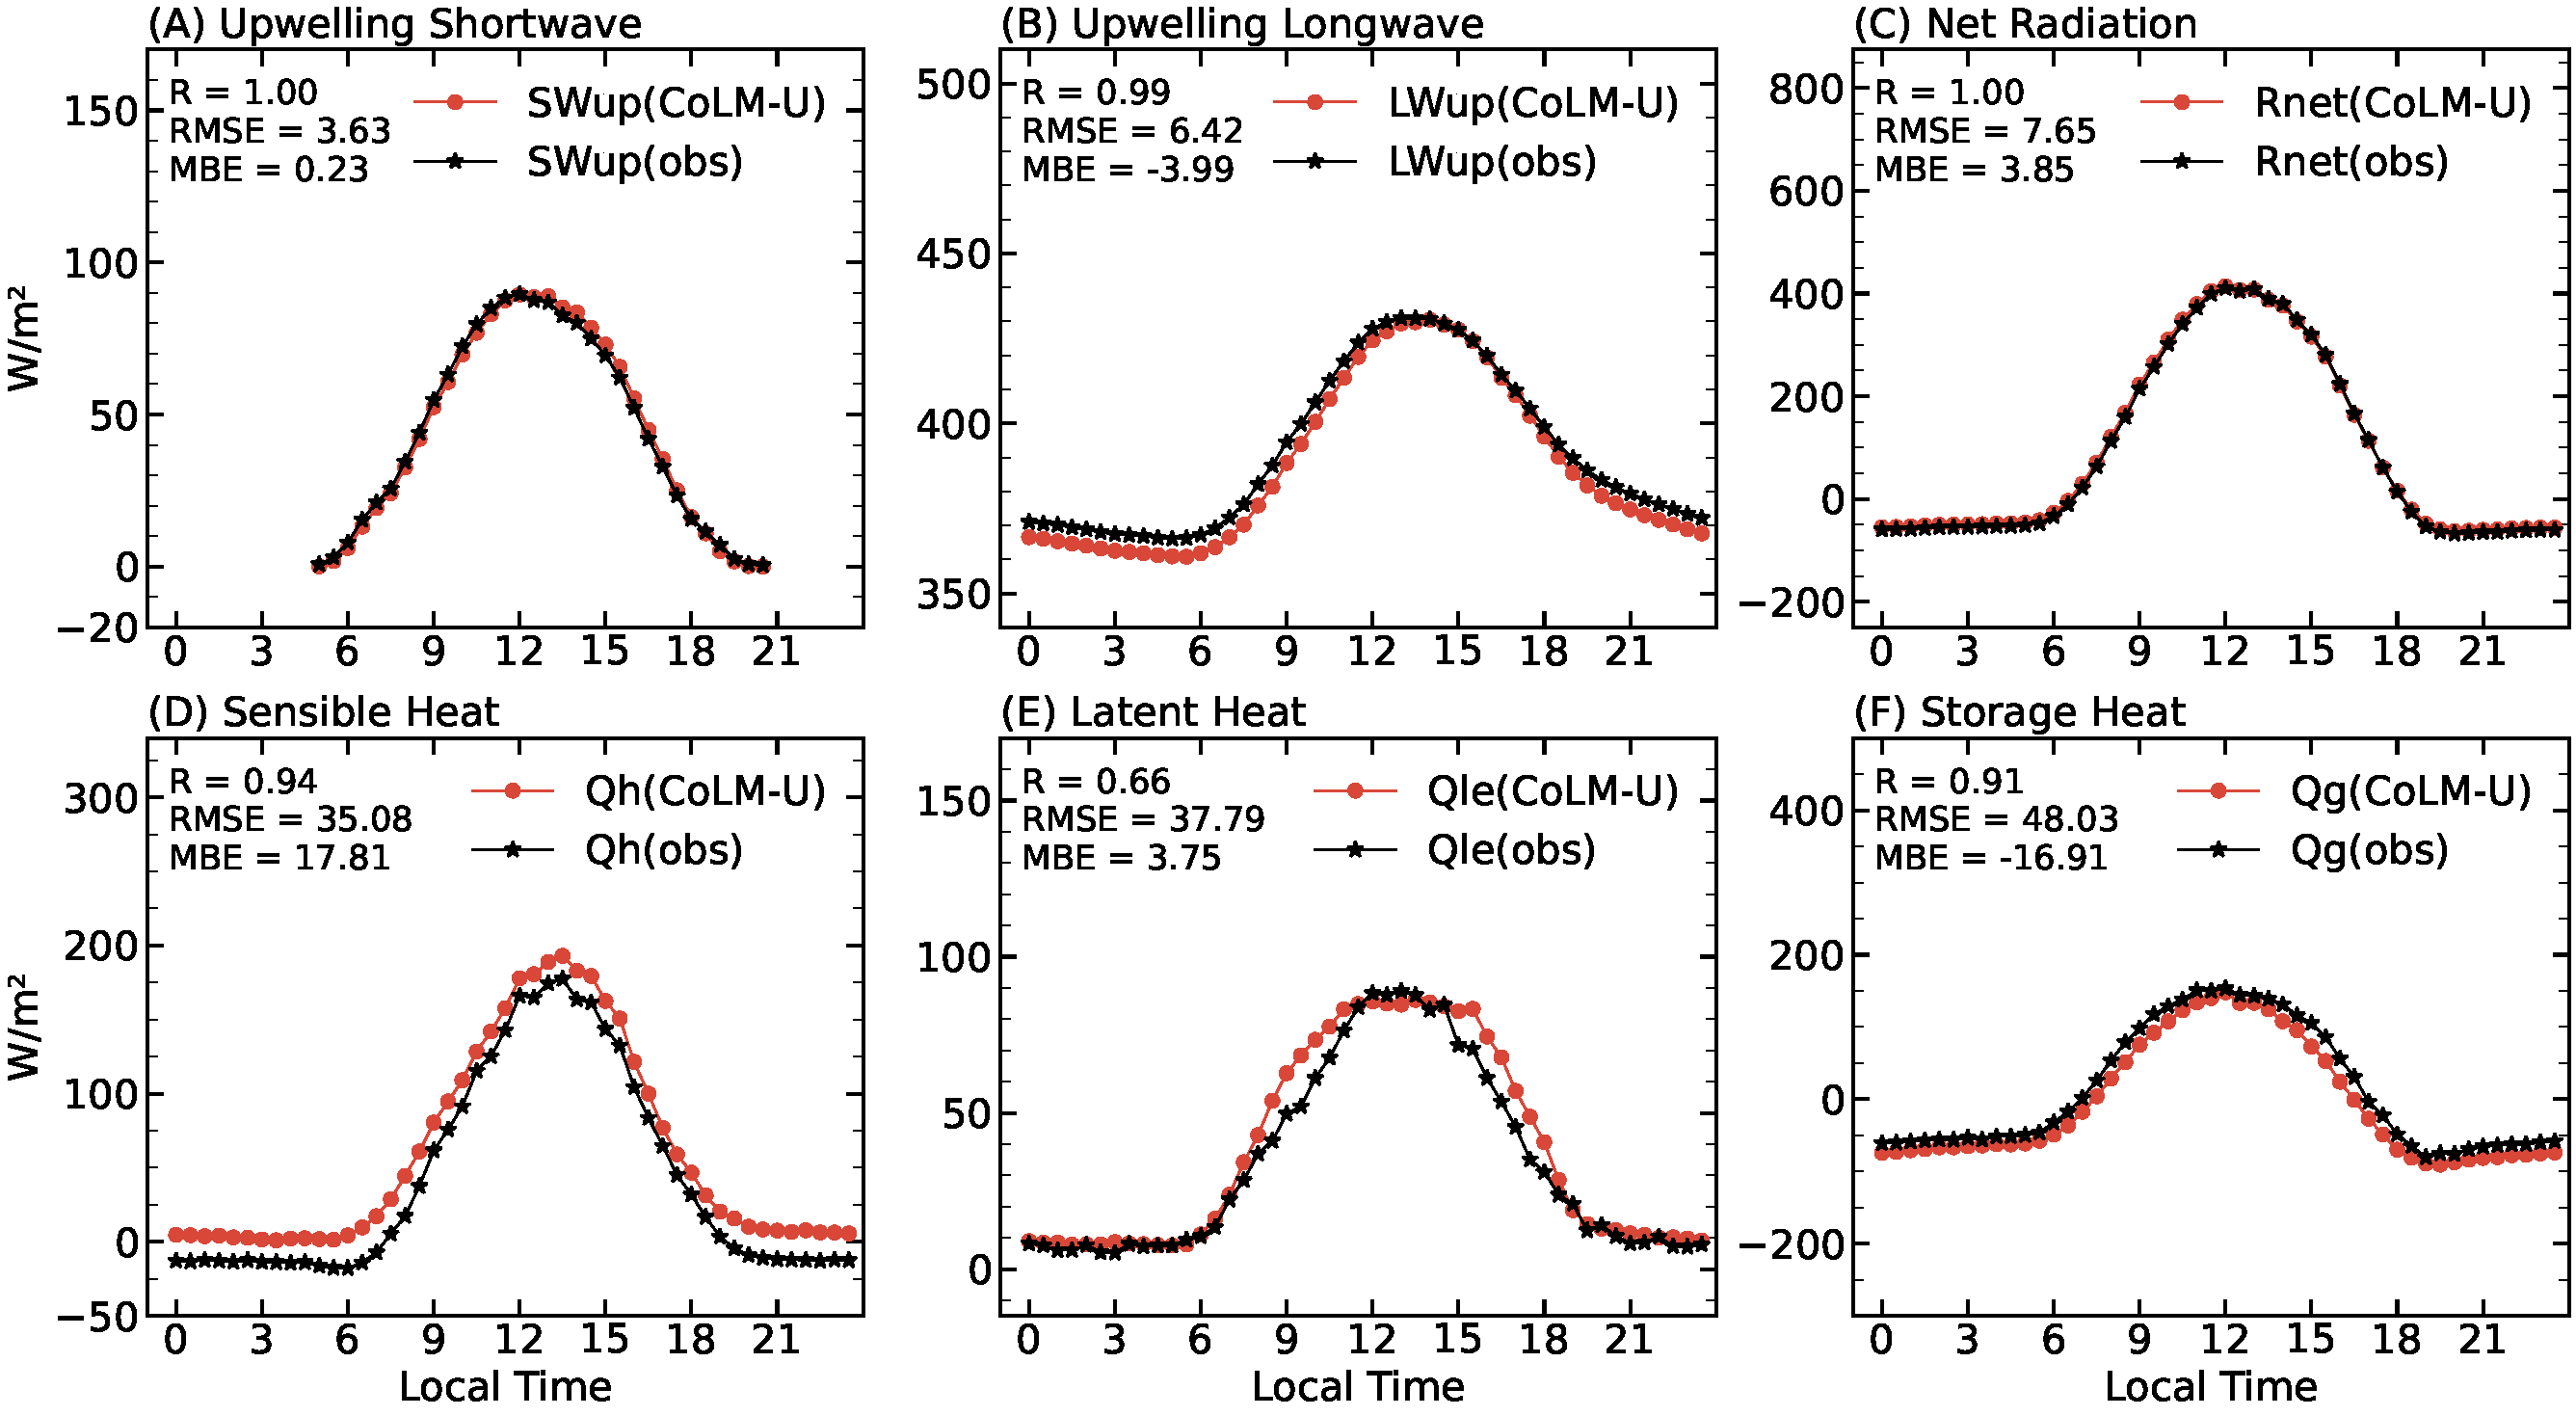
\includegraphics[width=0.90\textwidth]{figures/Example03_Site_AU-Preston.pdf}
    \caption{CoLM2024城市模型模拟AU-Preston站点向上短波、向上长波、净辐射、感热通量、潜热通量和储热通量平均日变化及其与观测对比结果(单位:\unit{W.m^{-2}})}
    \label{fig:fig_example03_au}
\end{figure}

\section{实例4:生物地球化学过程模拟}

本实例配置了一个常用的全球模拟的情景。实例使用了2.5\textdegree $\times$ 1.875\textdegree 的经纬度网格,植物功能类型(PFT)方案的植被结构次网格,以及van Genuchten-Mualem土壤水特征曲线模型,打开了CoLM2024的生物地球化学循环过程模块。本实例关于配置文件、重启数据、地表数据和驱动数据的简介已罗列在表~\ref{ex4table}中。

\begin{table}[htbp]
\caption{实例4配置文件和数据一览表}
\centering \renewcommand{\arraystretch}{1.5}
\label{ex4table}
\begin{tabular}{llc}
\toprule
\textbf{数据名} & \textbf{文件/目录名} & \textbf{是否需要解压缩} \\

\midrule

宏定义文件 & define.h & 否 \\
Namelist文件 & Global\_Grid\_2x2\_PC\_VG-BGC.nml & 否 \\
地表数据 & landdata.tar.gz & 是 \\
气象驱动数据 & crujra2.5.tar.gz & 是 \\
重启数据 & restart.tar.gz & 是 \\

\midrule

数据地址 & \multicolumn{2}{l}{大装置的地址}\\

\bottomrule
\end{tabular}
\end{table}

\subsection{实例4配置文件}\label{ex4config}

实例4的配置文件包含(1)\texttt{define.h}宏定义文件,控制模型大模块的开关,本实例的BGC开关通过宏定义文件控制; (2)Namelist文件,控制模拟实例的具体信息,本实例的宏定义文件和Namelist文件和实例1基本一致。其配置的主要差异包括:a)实例4的宏定义文件打开了BGC开关;b)并行化采用每12个进程一个工作组;c)叶面积指数无年际变化;d)所有碳氮库初始化时采用热启动;e)模拟分辨率和历史数据输出均改为经度2.5$\times$纬度1.875 。

\texttt{define.h}文件的内容为,
\lstinputlisting[language=fortran, basicstyle=\linespread{1.0}\footnotesize\ttfamily, commentstyle=\color{black}, numbers=left, numberstyle=\tiny, xleftmargin=1.5em,xrightmargin=0em, aboveskip=1em]{examples/bgc/define.h}

Namelist文件的内容为,
\lstinputlisting[language=fortran, basicstyle=\linespread{1.0}\footnotesize\ttfamily, commentstyle=\color{black}, numbers=left, numberstyle=\tiny, xleftmargin=1.5em,xrightmargin=0em, aboveskip=1em]{examples/bgc/Global_Grid_2x2_PC_VG_BGC.nml}

此实例中,\par
1)\textbf{并行化}方面,将全球分为20\textdegree$\times$20\textdegree 的数据块进行并行模拟(\texttt{DEF\_nx\_blocks=18}和\texttt{DEF\_ny\_blocks=9}),每12个进程为一个工作组,(\texttt{DEF\_PIO\_groupsize=12})。该最优每组进程数由大量实验测试得出。实例4分辨率相对实例1更粗,计算单元更少,因此最优每组进程数量较实例1下降;\par
2)\textbf{叶面积指数数据}使用了月变化数据(\texttt{DEF\_LAI\_MONTHLY=.true.}),且不随年份变化,仅使用2005年的叶面积指数(\texttt{DEF\_LAI\_CHANGE\_YEARLY=.false.});\par

3)对以下\textbf{过程参数化方案}进行了设置,此参数化方案与实例1完全一样:
\begin{itemize}[nosep,leftmargin=4em]
    \item 降水截留(\texttt{DEF\_Interception\_scheme=1});
    \item 土壤阻抗(\texttt{DEF\_RSS\_SCHEME=1});
    \item 土壤水运动数值方案(\texttt{DEF\_USE\_VariablySaturatedFlow=.true.});
    \item 过冷水方案(\texttt{DEF\_USE\_SUPERCOOL\_WATER=.true.});
    \item 产流参数化方案(\texttt{DEF\_Runoff\_SCHEME=3});
    \item 植被水力过程方案(\texttt{DEF\_USE\_PLANTHYDRAULICS=.true.});
    \item 水利用效率最优气孔方案(\texttt{DEF\_USE\_WUEST=.true.});
    \item 植物群落次网格简化方案(\texttt{DEF\_FAST\_PC=.true.});

\end{itemize}
\par

4)模型模拟的起始时间为2005年1月1日,模拟的结束时间为2005年12月31日 ;\par

5)模型模拟采用2.5 \textdegree $\times$ 1.875\textdegree 的经纬度网格(\texttt{DEF\_GRIDBASED\_lon\_res=2.5}和\texttt{DEF\_GRIDBASED\_lat\_res=1.875} ; \par

6)使用CRUJRA数据作为\textbf{大气驱动}(\texttt{DEF\_forcing\_namelist=<path>/CRUJRA.nml});\par

7)每年保存一次\textbf{重启动}文件(\texttt{DEF\_WRST\_FREQ=‘YEARLY’});\par

8)\textbf{历史数据的输出},
\begin{itemize}[nosep,leftmargin=4em]
    \item 为保持和模型分辨率一致,历史数据的空间分辨率也为2.5\textdegree $\times$ 1.875\textdegree 经纬度网格(\texttt{DEF\_hist\_lon\_res=2.5}和\texttt{DEF\_hist\_lon\_res=1.875});
    \item 输出变量的月值(\texttt{DEF\_HIST\_FREQ='MONTHLY'});
    \item 每月的数据保存在一个文件中(\texttt{DEF\_HIST\_groupby='MONTH'});
    \item 输出所有变量(\texttt{DEF\_hist\_vars\_out\_default=.true.}).
\end{itemize}\par

9)其他配置使用模式默认值。

\subsection{实例4地表数据}

实例4的地表数据和实例1的配置基本相同,区别主要在于分辨率,实例1的空间分辨率是0.5 \textdegree $\times$ 0.5\textdegree,而实例4有相对较粗的的空间分辨率,2.5 \textdegree $\times$ 1.875\textdegree。另外,由于BGC实验刻画的时间尺度相对更长(百年际),但叶面积指数数据覆盖时间仅为近20年,因此实例4的叶面积指数仅用2005年的气候态变化产品。除此之外,并行化配置,土壤水力参数、热力参数、叶面积指数、植被功能型覆盖比例、湖深、树高、地形和土壤质地等参数和实例1完全一致。

\subsection{实例4气象驱动数据}

实例4仍然使用Climate Research Unit and Japanese Reanalysis (CRUJRA) 2005年的气象驱动数据。本实例需要修改的案例Namelist文件和驱动Namelist文件(CRUJRA.nml),特别是CRUJRA驱动地址的设置见实例1(第~\ref{ex1forcing}节)的介绍。虽然实例4的空间分辨率与实例1并不一致,但驱动Namelist文件并不需要额外的修改。CRUJRA被CoLM读入后将根据模型设置进行时间和空间上的插值。

\subsection{实例4重启数据}

实例4的模拟初始于2005年1月1日,其重启数据由前序模拟生成。前序模拟的方案配置与~\ref{ex4config}节内容基本相同,但模拟时间从1850年1月1日开始到2004年12月31日结束。由于BGC模拟对初始状态十分敏感,所以需要在1850年时,进行长时间预热,本实验的预热包括100年半解析加速预热和30年普通自然预热,最后在1850年基本达到碳氮库的平衡状态。随后在1850年1月1日到2004年12月31日的过渡状态模拟结束后,得到实例4的重启数据。

\subsection{实例4操作步骤}

\textbf{第1步}:修改宏定义文件\texttt{define.h}

该文件位于源代码\texttt{include}目录下,可根据章节~\ref{ex4config} 进行修改,或者用本指南提供的宏定义文件进行覆盖。

\bigskip
\textbf{第2步}:建立实例运行Namelist文件

在源代码\texttt{run}目录下建立用于实例运行Namelist文件,可参考章节~\ref{ex4config} Namelist文件部分进行修改或者用本指南所提供的文件\texttt{Global\_Grid\_50km\_PC\_VG-BGC.nml}覆盖。

\bigskip
\textbf{第3步}:建立实例目录

用户新建实例目录,目录命名与Namelist文件的\texttt{DEF\_CASE\_NAME}设置保持一致,即Global\_Grid\_50km\_PC\_VG-BGC。本实例已提供地表数据,因此用户需手动建立实例目录。另外,需修改Namelist文件中的\texttt{DEF\_dir\_output}值为实例文件夹所在的目录(即父目录),例:实例目录的路径是 \texttt{/path/to/Global\_Grid\_50km\_PC\_VG-BGC},\texttt{DEF\_dir\_output}须设置为 \texttt{/path/to/}。

\bigskip
\textbf{第4步}:准备地表数据

解压指南所提供的本实例地表数据文件\texttt{landdata.tar.gz},解压后得到的文件夹\texttt{landdata}放置于实例目录下。

\bigskip
\textbf{第5步}:准备驱动数据

解压所提供的本实例驱动文件\texttt{crujra2.5-2005.tar.gz},首先修改驱动配置文件\texttt{CRUJRA.nml},该文件通常在\texttt{run/forcing}目录下。通过修改变量\texttt{DEF\_dir\_forcing}设置,指定驱动路径。最后,须确保Namelist文件中的\texttt{DEF\_forcing\_namelist}设置于驱动配置文件路径一致。

\bigskip
\textbf{第6步}:编译源代码

进入到源代码主目录,运行\texttt{make}命令进行编译,
\begin{quote}
\begin{lstlisting}
make
\end{lstlisting}
\end{quote}

\bigskip
\textbf{第7步}:运行初始化程序

本实例为用户提供了重启数据,可以依赖重启数据进行热启动。解压指南所提供的本实例重启数据文件\texttt{restart.tar.gz},解压后得到的文件夹\texttt{restart}放置于实例目录下。

\bigskip
\textbf{第8步}:执行主程序

在\texttt{run}目录下,执行
%\begin{quote}
\begin{lstlisting}[xleftmargin=2.5em]
mpirun -np $nproc ./colm.x Global_Grid_50km_PC_VG-BGC.nml
\end{lstlisting}
%\end{quote}

其中,\$nproc为实际使用的计算核心数。成功执行后,模式运行结果会在实例目录下的history文件夹中输出。


\subsection{实例4的模拟结果展示}

实例4中,CoLM2024的发布版本实现了2005年的全球2.5 \textdegree $\times$ 1.875\textdegree 分辨率的生物地球化学循环模拟,其中植物碳库(地上生物量和地下生物量的总和)全球空间分布模拟结果见图~\ref{fig:fig_example04_totvegc}。CoLM2024模型对2005年全球植物碳库分布与全球森林分布地图一致。其中,CoLM的植物碳库在赤道附近,尤其是亚马逊雨林,具有较高的模拟结果。副热带干旱区(如撒哈拉沙漠)受水分限制导致植物碳库几乎为0。中高纬度的北方森林区域的高植物碳库带也被CoLM2024清晰的模拟出。全球植物碳库、蒸散发和降水的纬向分布相似,模拟结果展现出CoLM植物生长的水利用特征。

\begin{figure}[htpb]
    \centering
    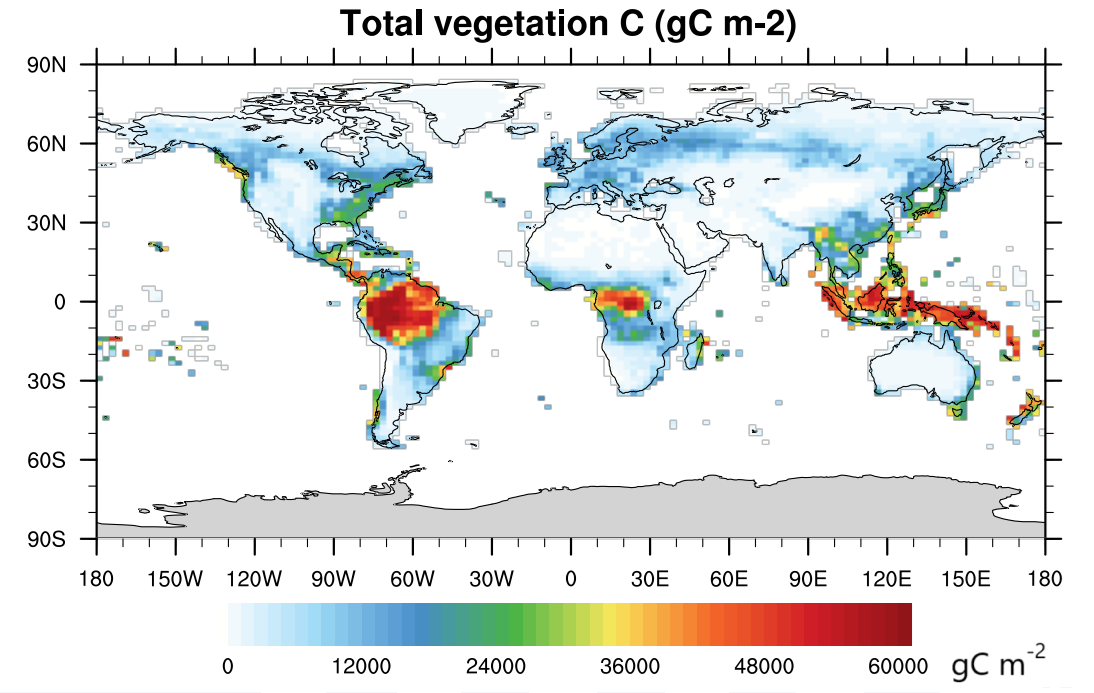
\includegraphics[width=0.90\textwidth]{figures/Example04_TotvegC_Global_Grid_2x2_PC_VG.png}
    \caption{CoLM2024生物地球化学循环模拟结果(2005年):植物碳库($\mathrm{gC \cdot m^{-2}}$)全球分布}
    \label{fig:fig_example04_totvegc}
\end{figure}

\section{实例5:区域高分辨率模拟与驱动数据降尺度}

本实例配置了一个区域高分辨率模拟情景。实例使用了1千米的经纬度网格,植物群落(PC)方案的植被结构次网格,以及van Genuchten-Mualem土壤水特征曲线模型,并使用MPI进行并行加速。本实例中,驱动数据的网格为1/4度,远大于模式网格(1/120度),因此,在模式运行过程中,对驱动数据进行了实时降尺度。

\begin{table}[htbp]
\caption{实例5配置文件和数据一览表}
\centering \renewcommand{\arraystretch}{1.5}
\label{ex5table}
\begin{tabular}{lp{0.4\textwidth}c}
\toprule
\textbf{数据名} & \textbf{文件/目录名} & \textbf{是否需要解压缩} \\\midrule

宏定义文件 & define.h & 否 \\
Namelist文件 & GreaterBay\_Grid\_1km\_PC\_VG.nml & 否 \\
模拟区域范围精细边界文件 & greaterbay\_1km\_filter.nc & 否\\
地形信息文件 & HResTopo.tar.gz,内含6个数据文件:slope.nc, aspect.nc, curvature.nc, sky\_view\_factor.nc, terrain\_elev\_angle\_back.nc, terrain\_elev\_angle\_front.nc & 是 \\
地表数据 & landdata.tar.gz & 是 \\
气象驱动数据 & ear5-2005.tar.gz & 是 \\
重启数据 & restart.tar.gz & 是 \\

\bottomrule
\end{tabular}
\end{table}

\subsection{实例5配置文件} \label{ex5config}
如表~\ref{ex5table} 所示,实例5的配置文件包含(1)宏定义文件define.h,为控制模型大模块的开关,完整介绍见第三部分第3节; (2)Namelist文件,为控制模拟实例的具体信息,完整介绍见第三部分第4节。

实例5的\texttt{define.h}文件的内容为,
\lstinputlisting[language=fortran, basicstyle=\linespread{1.0}\footnotesize\ttfamily, commentstyle=\color{black}, numbers=left, numberstyle=\tiny, xleftmargin=1.5em,xrightmargin=0em, aboveskip=1em]{examples/hires/define.h}

实例5的Namelist文件的内容为,
\lstinputlisting[language=fortran, basicstyle=\linespread{1.0}\footnotesize\ttfamily, commentstyle=\color{black}, numbers=left, numberstyle=\tiny, xleftmargin=1.5em,xrightmargin=0em, aboveskip=1em]{examples/hires/GreaterBay_Grid_1km_PC_VG.nml}

此实例中,\par
1)区域大致范围通过\texttt{DEF\_domain}进行设定,并使用文件\texttt{DEF\_file\_mesh\_filter}中的'mesh\_filter'变量进一步细化需要模拟的\textbf{区域范围};\par
2)\textbf{并行化}方面,将全球分为180\textdegree$\times$90\textdegree 的数据块进行并行模拟(\texttt{DEF\_nx\_blocks}和\texttt{DEF\_ny\_blocks}),每24个进程为一个工作组(\texttt{DEF\_PIO\_groupsize});\par
3)\textbf{过程参数化方案}均使用模式默认值;\par
4)使用ERA5数据作为\textbf{大气驱动}(\texttt{DEF\_forcing\_namelist});\par
5)从粗分辨率的驱动数据到细分辨率的陆表单元使用\textbf{双线性插值}的方法\\ (\texttt{DEF\_Forcing\_Interp\_Method}),在插值的过程中同时进行\textbf{降尺度}\\ (\texttt{DEF\_USE\_Forcing\_Downscaling});\par
6)\textbf{降尺度方法}中,对降水的调整使用Liston and Elder~(2006)提出的方案\\ (\texttt{DEF\_DS\_precipitation\_adjust\_scheme}),对下行长波辐射的调整使用van Tricht et al. (2016)提出的方案(\texttt{DEF\_DS\_longwave\_adjust\_scheme});\par
7)每月保存一次\textbf{重启动}变量(\texttt{DEF\_WRST\_FREQ});\par
8)\textbf{历史数据的输出},
\begin{itemize}[nosep,leftmargin=4em]
    \item 输出到1千米经纬度网格(\texttt{DEF\_hist\_lon\_res}和\texttt{DEF\_hist\_lon\_res});
    \item 输出变量的日值(\texttt{DEF\_HIST\_FREQ});
    \item 每月的数据保存在一个文件中(\texttt{DEF\_HIST\_groupby});
    \item 输出所有变量(\texttt{DEF\_hist\_vars\_out\_default}).
\end{itemize}\par
9)其他配置使用模式默认值。

\subsection{实例5数据}

实例5模拟的是一个区域(21.5\textdegree N\textasciitilde 24.5\textdegree N, 111.0\textdegree E\textasciitilde 115.5\textdegree E)内的陆面过程,但其地表数据的制作仍基于全球原始数据。为了提高并行效率,地表制作程序将全球区域分为经向180个×纬向90个数据块,每个数据块最多包含120×120个网格单元。实例5使用了数据文件\texttt{DEF\_file\_mesh\_filter}对模拟区域的边界进行进一步的描述,文件中包含定义在经纬度网格上的变量`mesh\_filter',其值大于0时,表示对这个网格单元进行模拟,否则将不模拟。

另外,驱动数据降尺度使用的主要数据为地形信息,包括坡度、坡向、天空可视因子和地形高度角等。

\begin{figure}[htpb]
    \centering
    \includegraphics[width=0.90\textwidth]{figures/Example05_BilinearDownscaling.pdf}
    \includegraphics[width=0.90\textwidth]{figures/Example05_BilinearOnly.pdf}
    \caption{高分辨率模拟实例5中,(a)使用降尺度方法和(b)不使用降尺度方法对驱动数据中的气温进行重采样的结果。图中实线为驱动数据网格(0.25度经纬度网格)}
    \label{fig:fig_hiresdownscaling}
\end{figure}

\subsection{实例5操作步骤}

\textbf{第1步}:修改宏定义文件\texttt{define.h}

该文件位于源代码\texttt{include}目录下,可根据章节~\ref{ex5config} 进行修改,或者用本指南提供的宏定义文件(见表\ref{ex5table})进行覆盖。

\bigskip
\textbf{第2步}:建立实例运行Namelist文件

在任意目录下建立用于实例运行的Namelist文件,可参考章节~\ref{ex5config} Namelist文件部分进行修改或者用本指南所提供的文件\texttt{GreaterBay\_Grid\_1km\_PC\_VG.nml}覆盖。

\bigskip
\textbf{第3步}:建立实例目录

用户新建实例目录,目录命名与Namelist文件的\texttt{DEF\_CASE\_NAME}设置保持一致(本例中即GreaterBay\_Grid\_1km\_PC\_VG)。本实例已提供地表数据,因此用户需手动建立实例目录。另外,需修改Namelist文件中的\texttt{DEF\_dir\_output}值为实例文件夹所在的目录(即父目录),比如:实例目录的路径是/path/to/GreaterBay\_Grid\_1km\_PC\_VG,则\texttt{DEF\_dir\_output}须设置为/path/to/。

\bigskip
\textbf{第4步}:准备地表数据

解压指南所提供的本实例地表数据文件\texttt{landdata.tar.gz},解压后得到的文件夹\texttt{landdata}放置于实例目录下。

\bigskip
\textbf{第5步}:准备区域范围数据和地形数据

在Namelist文件中修改变量DEF\_file\_mesh\_filter指向区域范围精细边界文件greaterbay\_1km\_filter.nc的路径。

解压放置地形信息文件HResTopo.tar.gz,在Namelist文件中修改变量DEF\_DS\_\allowbreak HiresTopographyDataDir指向其存放路径。

\bigskip
\textbf{第6步}:准备驱动数据

解压指南所提供的本实例驱动文件\texttt{ear5-2005.tar.gz},修改解压后的驱动配置文件\texttt{ERA5.nml}(位于源代码目录的run/forcing文件夹下):通过修改变量\texttt{DEF\_dir\_forcing}设置,指定驱动路径。最后,须确保Namelist文件中的\texttt{DEF\_forcing\_namelist}指向驱动配置文件\texttt{ERA5.nml}的路径。

\bigskip
\textbf{第7步}:编译源代码

进入到源代码主目录,运行\texttt{make}命令进行编译,
\begin{quote}
\begin{lstlisting}
make
\end{lstlisting}
\end{quote}

\bigskip
\textbf{第8步}:运行初始化程序

本实例为用户提供了重启数据,可以依赖重启数据进行启动。解压指南所提供的本实例重启数据文件\texttt{restart.tar.gz},解压后得到的文件夹\texttt{restart}放置于实例目录下。

用户也可在run目录下执行以下命令自己制作重启动数据,
\begin{quote}
\begin{lstlisting}
mpirun -np $nproc ./mkinidata.x GreaterBay_Grid_1km_PC_VG.nml
\end{lstlisting}
\end{quote}
其中,\$nproc为实际使用的计算核心数。

\bigskip
\textbf{第9步}:执行主程序

在\texttt{run}目录下,执行
\begin{quote}
\begin{lstlisting}
mpirun -np $nproc ./colm.x GreaterBay_Grid_1km_PC_VG.nml
\end{lstlisting}
\end{quote}
其中,\$nproc为实际使用的计算核心数。成功执行后,模式运行结果会在实例目录下的history文件夹中输出。

\subsection{实例5模拟结果}

实例5中演示了CoLM2024中的降尺度方法。CoLM2024允许模式单元和大气驱动数据定义在不同的经纬度网格上,由大气驱动数据到模式单元的插值映射可使用面积加权平均,也可以使用双线性插值。实例5中,驱动数据的分辨率为0.25度,模式单元的分辨率为1公里。若仅使用双线性插值,对近地面气温插值映射的结果见图\ref{fig:fig_hiresdownscaling}(b),尽管分辨率得到了提升,但有效信息并未增加。若使用双线性插值的同时,对驱动数据进行降尺度(见图\ref{fig:fig_hiresdownscaling}(a)),则可融合地形数据,在提升分辨率的同时,进一步增加有效信息。



\section{实例6:流域单元和侧向流模拟}

本节配置了一个基于流域网格单元并包含侧向流模拟的实例。实例使用了流域单元网格并打开了侧向流模块,使用基于植被群落(PC)的植被结构次网格,以及van Genuchten-Mualem土壤水特征曲线模型,并基于MPI进行并行加速。其配置文件和数据信息如表~\ref{ex6table} 所示。

\begin{table}[htbp]
\caption{实例6配置文件和数据一览表}
\centering \renewcommand{\arraystretch}{1.5}
\label{ex6table}
\begin{tabular}{lcc}
\toprule
\textbf{数据名} & \textbf{文件/目录名} & \textbf{是否需要解压缩} \\\midrule
宏定义文件 & define.h & 否 \\
Namelist文件 & PearlRiver\_Catch\_250km2\_PC\_VG .nml & 否 \\
流域单元网格文件 & PearlRiver\_250km2.nc & 否\\
网格单元信息文件 & PearlRiver\_250km2.nc & 否 \\
地表数据 & landdata.tar.gz & 是 \\
气象驱动数据 & ear5-2003-2005.tar.gz & 是 \\
重启数据 & restart.tar.gz & 是 \\

\bottomrule
\end{tabular}
\end{table}

\subsection{实例6配置文件}\label{ex6config}
实例6的配置文件包含(1)宏定义文件define.h,为控制模型大模块的开关,完整介绍见第三部分第3节;(2)Namelist文件,为控制模拟实例的具体信息,完整介绍见第三部分第4节。

实例6中\texttt{define.h}文件的内容为,
\lstinputlisting[language=fortran, basicstyle=\linespread{1.0}\footnotesize\ttfamily, commentstyle=\color{black}, numbers=left, numberstyle=\tiny, xleftmargin=1.5em,xrightmargin=0em, aboveskip=1em]{examples/catchment/define.h}

Namelist文件的内容为,
\lstinputlisting[language=fortran, basicstyle=\linespread{1.0}\footnotesize\ttfamily, commentstyle=\color{black}, numbers=left, numberstyle=\tiny, xleftmargin=1.5em,xrightmargin=0em, aboveskip=1em]{examples/catchment/PearlRiver_Catch_250km2_PC_VG.nml}

此实例中,\par
1)区域大致范围通过\texttt{DEF\_domain}进行设定;\par
2)从文件\texttt{DEF\_CatchmentMesh\_data}中的`icatchment2d'和`ihydrounit2d'变量读入\textbf{描述单元划分的数据};\par
3)文件\texttt{DEF\_ElementNeighbour\_file}中的数据描述了\textbf{侧向流模拟}所需的流域单元及单元之间的参数信息;\par
4)\textbf{并行化}方面,将全球分为5\textdegree$\times$ 5\textdegree 的数据块进行并行模拟(\texttt{DEF\_nx\_blocks}和\texttt{DEF\_ny\_blocks}),每24个进程为一个工作组(\texttt{DEF\_PIO\_groupsize});\par
5)\textbf{地表覆盖类型数据}使用了2005年的数据(\texttt{DEF\_LC\_YEAR});\par
6)\textbf{叶面积指数数据}使用了2005年的月数据(不随年份变化时,叶面积指数数据的年份同\texttt{DEF\_LC\_YEAR}),不随年份变化(\texttt{DEF\_LAI\_CHANGE\_YEARLY});\par
7)使用FIT算法进行\textbf{土壤水热参数升尺度}(\texttt{DEF\_USE\_SOILPAR\_UPS\_FIT});\par
8)使用水体深度动态变化方案(\texttt{DEF\_USE\_Dynamic\_Lake}),其余\textbf{过程参数化方案}均使用模式默认值;\par
9)使用ERA5数据作为\textbf{大气驱动}(\texttt{DEF\_forcing\_namelist});\par
10)每月保存一次\textbf{重启动}变量(\texttt{DEF\_WRST\_FREQ});\par
11)\textbf{历史数据的输出},
\begin{itemize}[nosep,leftmargin=4em]
    \item 输出到0.05\textdegree 经纬度网格(\texttt{DEF\_hist\_lon\_res}和\texttt{DEF\_hist\_lon\_res});
    \item 输出变量的日值(\texttt{DEF\_HIST\_FREQ});
    \item 每月的数据保存在一个文件中(\texttt{DEF\_HIST\_groupby});
    \item 输出所有变量(\texttt{DEF\_hist\_vars\_out\_default}).
\end{itemize}\par
12)其他配置使用模式默认值。

\subsection{实例6数据}

\begin{figure}[htpb]
    \centering
    \includegraphics[width=\textwidth]{figures/Example06_PearlRiverMesh.pdf}
    \caption{基于流域单元网格对珠江流域进行模拟时的流域单元划分图。本实例中,流域单元的面积阈值为250 \unit{km^2}。}
    \label{fig:fig_pearlriver}
\end{figure}

实例6基于流域单元网格,模拟珠江流域的陆面过程。其地表数据的制作仍基于全球原始数据。为了提高并行效率,地表制作程序将全球区域分为经向72个×纬向36个数据块。实例6中流域单元的划分数据来自文件\texttt{DEF\_CatchmentMesh\_data},其包含两个基于90米分辨率的变量:变量`icatchment2d'标记了每个90米的格点所在的流域单元,变量`ihydrounit2d'标记了每个90米的格点所属的高度带单元。流域单元的划分结果见图~\ref{fig:fig_pearlriver}。

实例6基于流域单元网格对侧向流过程进行了模拟(开关为宏定义文件中的\texttt{\#define CatchLateralFlow})。进行侧向流模拟时,还需模式单元的相邻关系、边界长度等信息,这些数据放置于文件\texttt{DEF\_ElementNeighbour\_file}中。

\subsection{实例6操作步骤}

\textbf{第1步}:修改宏定义文件\texttt{define.h}

该文件位于源代码\texttt{include}目录下,可根据章节~\ref{ex6config} 进行修改,或者用本指南提供的宏定义文件(见表\ref{ex6table})进行覆盖。

\bigskip
\textbf{第2步}:建立实例运行Namelist文件

在任意目录下建立用于实例运行的Namelist文件,可参考章节~\ref{ex6config} Namelist文件部分进行修改或者用本指南所提供的文件\texttt{PearlRiver\_Catch\_250km2\_PC\_VG.nml}覆盖。

\bigskip
\textbf{第3步}:建立实例目录

用户新建实例目录,目录命名与Namelist文件的\texttt{DEF\_CASE\_NAME}设置保持一致(本例中即PearlRiver\_Catch\_250km2\_PC\_VG)。本实例已提供地表数据,因此用户需手动建立实例目录。另外,需修改Namelist文件中的\texttt{DEF\_dir\_output}值为实例文件夹所在的目录(即父目录),比如:实例目录的路径是/path/to/PearlRiver\_Catch\_250km2\_PC\_VG,则\texttt{DEF\_dir\_output}须设置为/path/to/。

\bigskip
\textbf{第4步}:准备地表数据

解压指南所提供的本实例地表数据文件\texttt{landdata.tar.gz},解压后得到的文件夹\texttt{landdata}放置于实例目录下。

\bigskip
\textbf{第5步}:准备区域流域网格和单元信息数据

在Namelist文件中修改变量DEF\_CatchmentMesh\_data指向流域网格信息文件PearlRiver\_250km2.nc的路径。

在Namelist文件中修改变量DEF\_ElementNeighbour\_file指向网格单元信息文件PearlRiver\_250km2.nc的路径。

\bigskip
\textbf{第6步}:准备驱动数据

解压指南所提供的本实例驱动文件\texttt{ear5-2003-2005.tar.gz},修改解压后的驱动配置文件\texttt{ERA5.nml}(位于源代码目录的run/forcing文件夹下):修改变量\texttt{DEF\_dir\_forcing}指定驱动数据路径。最后,须确保Namelist文件中的\texttt{DEF\_forcing\_namelist}指向驱动配置文件\texttt{ERA5.nml}的路径。

\bigskip
\textbf{第7步}:编译源代码

进入到源代码主目录,运行\texttt{make}命令进行编译,
\begin{quote}
\begin{lstlisting}
make
\end{lstlisting}
\end{quote}

\bigskip
\textbf{第8步}:运行初始化程序

本实例为用户提供了重启数据,可以依赖重启数据进行启动。解压指南所提供的本实例重启数据文件\texttt{restart.tar.gz},解压后得到的文件夹\texttt{restart}放置于实例目录下。

用户也可在run目录下执行以下命令自己制作重启动数据,
\begin{quote}
\begin{lstlisting}
mpirun -np $nproc ./mkinidata.x PearlRiver_Catch_250km2_PC_VG.nml
\end{lstlisting}
\end{quote}
其中,\$nproc为实际使用的计算核心数。

\bigskip
\textbf{第9步}:执行主程序

在\texttt{run}目录下,执行
\begin{quote}
\begin{lstlisting}
mpirun -np $nproc ./colm.x PearlRiver_Catch_250km2_PC_VG.nml
\end{lstlisting}
\end{quote}
其中,\$nproc为实际使用的计算核心数。成功执行后,模式运行结果会在实例目录下的history文件夹中输出。

\subsection{实例6模拟结果}

图\ref{fig:fig_pearlriver_discharge}展示了实例6中CoLM2024对珠江流域石角、梧州两个水文站点处径流所做的预报结果。尽管模型从2003年启动,只进行了1年时间的预热,且参数均为默认值,CoLM2024仍能较好地反映径流的变化,对径流量的预测也与观测基本吻合。

\begin{figure}[htpb]
    \centering
    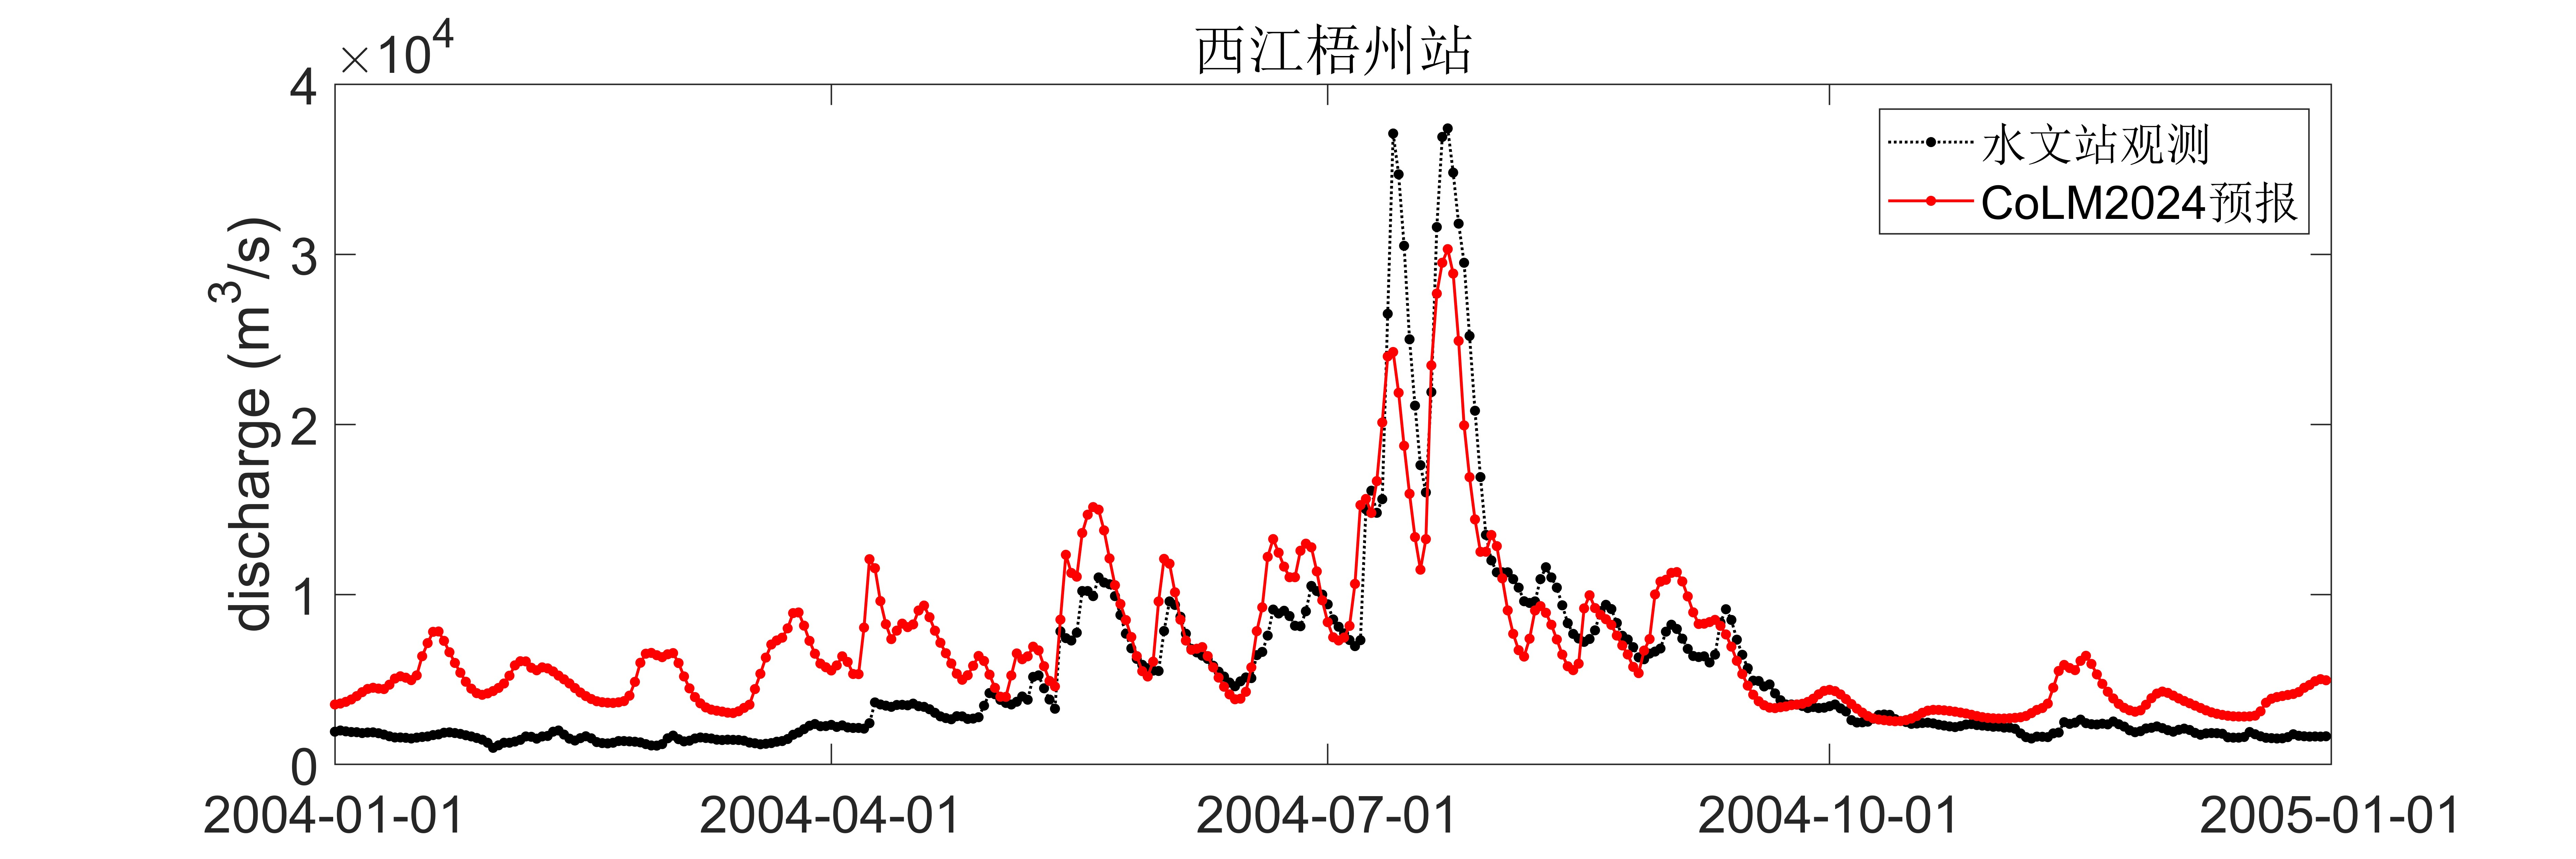
\includegraphics[width=\textwidth]{figures/Example06_pearl_wuzhou_discharge.jpg}
    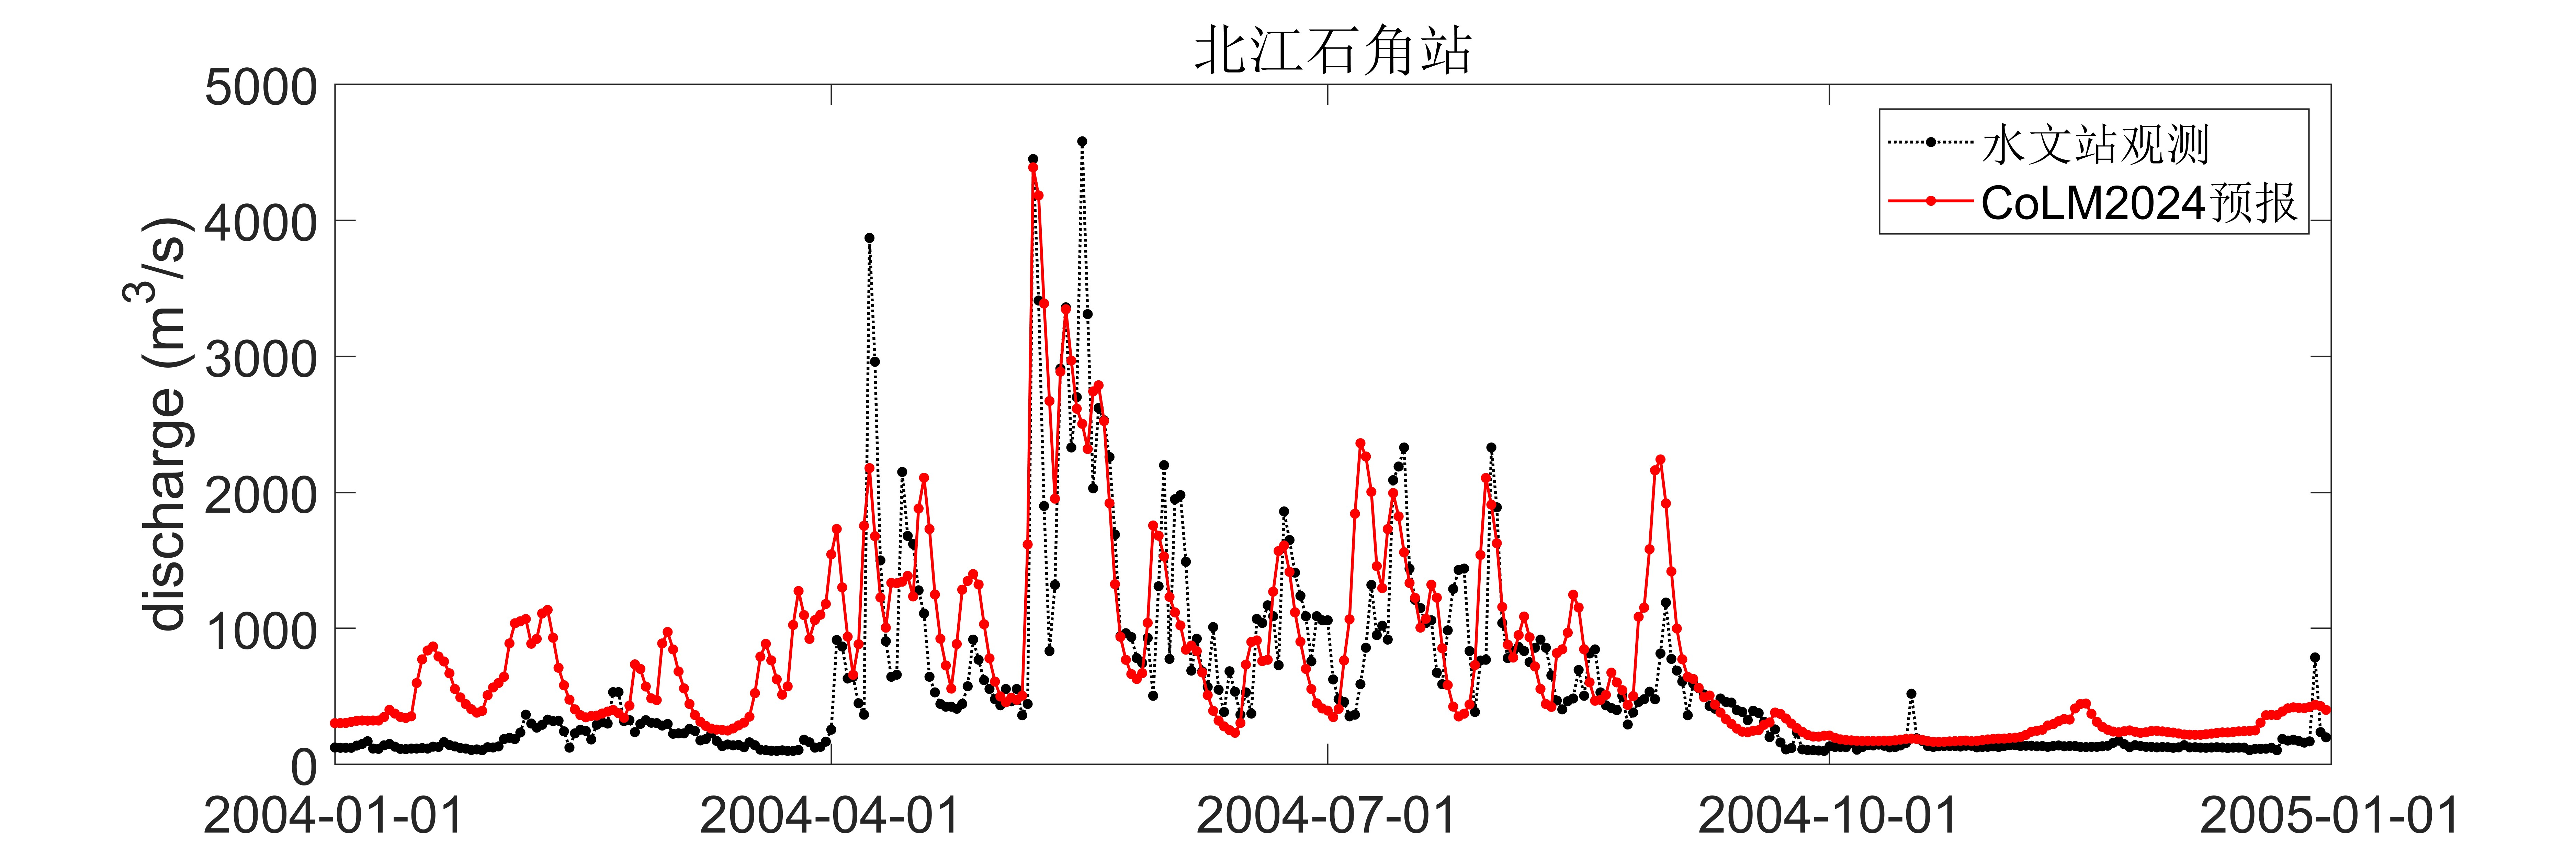
\includegraphics[width=\textwidth]{figures/Example06_pearl_shijiao_discharge.jpg}
    \caption{实例6:对珠江流域石角、梧州两个水文站点处径流的观测及CoLM2024的预报.}
    \label{fig:fig_pearlriver_discharge}
\end{figure}

\section{实例7:非结构网格单元模拟}

实例7采用蜂窝六边形离散格网(非结构网格)作为模型构建基础单元,非结构网格的制作基于全球原始数据,使用自主开发的自适应网格技术,根据高分辨率高程、坡度、土地利用、植被类型等多种分布特征数据,自动生成基于多种特征的可变分辨率的非结构网格。模式运行采用过了基于植物群落次网格 (PC)的植被结构次网格,以及van Genuchten-Mualem土壤水特征曲线模型,并基于MPI进行并行加速。

\begin{table}[htbp]
\caption{实例7配置文件和数据一览表}
\centering \renewcommand{\arraystretch}{1.5}
\label{ex7table}
\begin{tabular}{lcc}
\toprule
\textbf{数据名} & \textbf{文件/目录名} & \textbf{是否需要解压缩} \\\midrule
宏定义文件 & define.h & 否 \\
Namelist文件 & PearlRiver\_unstr\_2500km2\_IGBP\_VG.nml & 否 \\
非结构网格文件 & PearlRiver\_patchtype\_NXP0144\_mode6.nc4 & 否\\
地表数据 & unstr\_landdata.tar.gz & 是 \\
气象驱动数据 & JRA55-2000-2010.tar.gz & 是 \\
重启数据 & unstr\_restart.tar.gz & 是 \\
输出数据 & unstr\_history.tar.gz & 是 \\

\bottomrule
\end{tabular}
\end{table}
\subsection{实例7配置文件}\label{ex7config}
实例7的配置文件包含(1)宏定义文件define.h,为控制模型大模块的开关,完整介绍见第三部分第3节;(2)Namelist文件,为控制模拟实例的具体信息,完整介绍见第三部分第4节。

实例7中\texttt{define.h}文件的内容为,
\lstinputlisting[language=fortran, basicstyle=\linespread{1.0}\footnotesize\ttfamily, commentstyle=\color{black}, numbers=left, numberstyle=\tiny, xleftmargin=1.5em,xrightmargin=0em, aboveskip=1em]{examples/unstructured/define.h}

Namelist文件的内容为,
\lstinputlisting[language=fortran, basicstyle=\linespread{1.0}\footnotesize\ttfamily, commentstyle=\color{black}, numbers=left, numberstyle=\tiny, xleftmargin=1.5em,xrightmargin=0em, aboveskip=1em]{examples/unstructured/PearlRiver_unstr_2500km2_IGBP_VG.nml}

此实例中,\par
1)区域大致范围通过\texttt{DEF\_domain}进行设定;\par
2)从文件\texttt{DEF\_file\_mesh}中的`elmindex'变量读入\textbf{描述单元划分的数据};\par
3)\textbf{地表覆盖类型数据}使用了2005年的数据(\texttt{DEF\_LC\_YEAR});\par
4)\textbf{叶面积指数数据}使用了2005年的月数据(不随年份变化时,叶面积指数数据的年份同\texttt{DEF\_LC\_YEAR}),不随年份变化(\texttt{DEF\_LAI\_CHANGE\_YEARLY});\par
5)使用FIT算法进行\textbf{土壤水热参数升尺度}(\texttt{DEF\_USE\_SOILPAR\_UPS\_FIT});\par
9)使用JRA55数据作为\textbf{大气驱动}(\texttt{DEF\_forcing\_namelist});\par
6)每月保存一次\textbf{重启动}变量(\texttt{DEF\_WRST\_FREQ});\par
7)\textbf{历史数据的输出},
\begin{itemize}[nosep,leftmargin=4em]
    \item 输出到0.05\textdegree 经纬度网格(\texttt{DEF\_hist\_lon\_res}和\texttt{DEF\_hist\_lon\_res});
    \item 输出变量的日值(\texttt{DEF\_HIST\_FREQ});
    \item 每月的数据保存在一个文件中(\texttt{DEF\_HIST\_groupby});
    \item 输出所有变量(\texttt{DEF\_hist\_vars\_out\_default}).
\end{itemize}\par
12)其他配置使用模式默认值。


\subsection{实例7数据}

\begin{figure}[htpb]
    \centering
    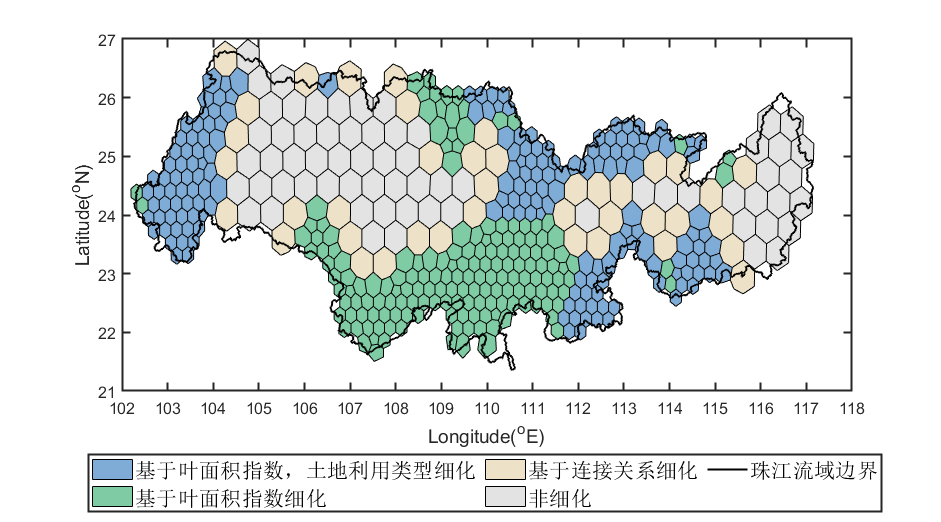
\includegraphics[width=\textwidth]{figures/Example07_PearlRiver_unstr_Mesh.jpg}
    \caption{珠江流域基于土地类型以及叶面积指数进行单次细化生成的非结构网格示意图。本实例中,土地类型的数量阈值为~10,叶面积指数的标准差阈值为~1.1}
    \label{fig:fig_pearlriver_unstr}
\end{figure}

实例7基于蜂窝六边形离散格网格,模拟珠江流域的陆面过程。其地表数据的制作仍基于全球原始数据,本
实验采用土地类型数量、叶面积指数均方根误差作为细化阈值,对所选区域内网格进行单次细化。实例7中网格划分数据来自文件~DEF\_file\_mesh,其包含变量`elmindex',标记了每个500米的基础格点所属的网格编号。六边形网格的划分结果见图~\ref{fig:fig_pearlriver_unstr}。
\subsection{实例7操作步骤}
\textbf{第1步}:修改宏定义文件\texttt{define.h}

该文件位于源代码\texttt{include}目录下,可根据章节~\ref{ex7config} 进行修改,或者用本指南提供的宏定义文件(见表\ref{ex7table})进行覆盖。

\bigskip
\textbf{第2步}:建立实例运行Namelist文件

在任意目录下建立用于实例运行的Namelist文件,可参考章节~\ref{ex7config} Namelist文件部分进行修改或者用本指南所提供的文件\texttt{PearlRiver\_unstr\_250km2\_IGBP\_VG.nml}覆盖。

\bigskip
\textbf{第3步}:建立实例目录

用户新建实例目录,目录命名与Namelist文件的\texttt{DEF\_CASE\_NAME}设置保持一致(本例中即PearlRiver\_Unstr\_250km2\_PC\_VG)。本实例已提供地表数据,因此用户需手动建立实例目录。另外,需修改Namelist文件中的\texttt{DEF\_dir\_output}值为实例文件夹所在的目录(即父目录),比如:实例目录的路径是/path/to/PearlRiver\_Unstr\_250km2\_PC\_VG,则\texttt{DEF\_dir\_output}须设置为/path/to/。

\bigskip
\textbf{第4步}:准备地表数据

解压指南所提供的本实例地表数据文件\texttt{landdata.tar.gz},解压后得到的文件夹\texttt{landdata}放置于实例目录下。

\bigskip
\textbf{第5步}:准备非结构网格信息数据

在Namelist文件中修改变量DEF\_file\_mesh指向非结构网格信息数据文件PearlRiver\_patchtype\_NXP0144\_mode6.nc的路径。

\bigskip
\textbf{第6步}:准备驱动数据

解压指南所提供的本实例驱动文件\texttt{JRA55-2003-2005.tar.gz},修改解压后的驱动配置文件\texttt{JRA55.nml}(位于源代码目录的run/forcing文件夹下):修改变量\texttt{DEF\_dir\_forcing}指定驱动数据路径。最后,须确保Namelist文件中的\texttt{DEF\_forcing\_namelist}指向驱动配置文件\texttt{JRA55.nml}的路径。

\bigskip
\textbf{第7步}:编译源代码

进入到源代码主目录,运行\texttt{make}命令进行编译,
\begin{quote}
\begin{lstlisting}
make
\end{lstlisting}
\end{quote}

\bigskip
\textbf{第8步}:运行初始化程序

本实例为用户提供了重启数据,可以依赖重启数据进行启动。解压指南所提供的本实例重启数据文件\texttt{restart.tar.gz},解压后得到的文件夹\texttt{restart}放置于实例目录下。

用户也可在run目录下执行以下命令自己制作重启动数据,
\begin{quote}
\begin{lstlisting}
mpirun -np $nproc ./mkinidata.x PearlRiver_unstr_250km2_IGBP_VG.nml
\end{lstlisting}
\end{quote}
其中,\$nproc为实际使用的计算核心数。

\bigskip
\textbf{第9步}:执行主程序

在\texttt{run}目录下,执行
\begin{quote}
\begin{lstlisting}
mpirun -np $nproc ./colm.x PearlRiver_unstr_250km2_IGBP_VG.nml
\end{lstlisting}
\end{quote}
其中,\$nproc为实际使用的计算核心数。成功执行后,模式运行结果会在实例目录下的history文件夹中输出。

\subsection{实例7模拟结果}


\begin{figure}[htpb]
    \centering
    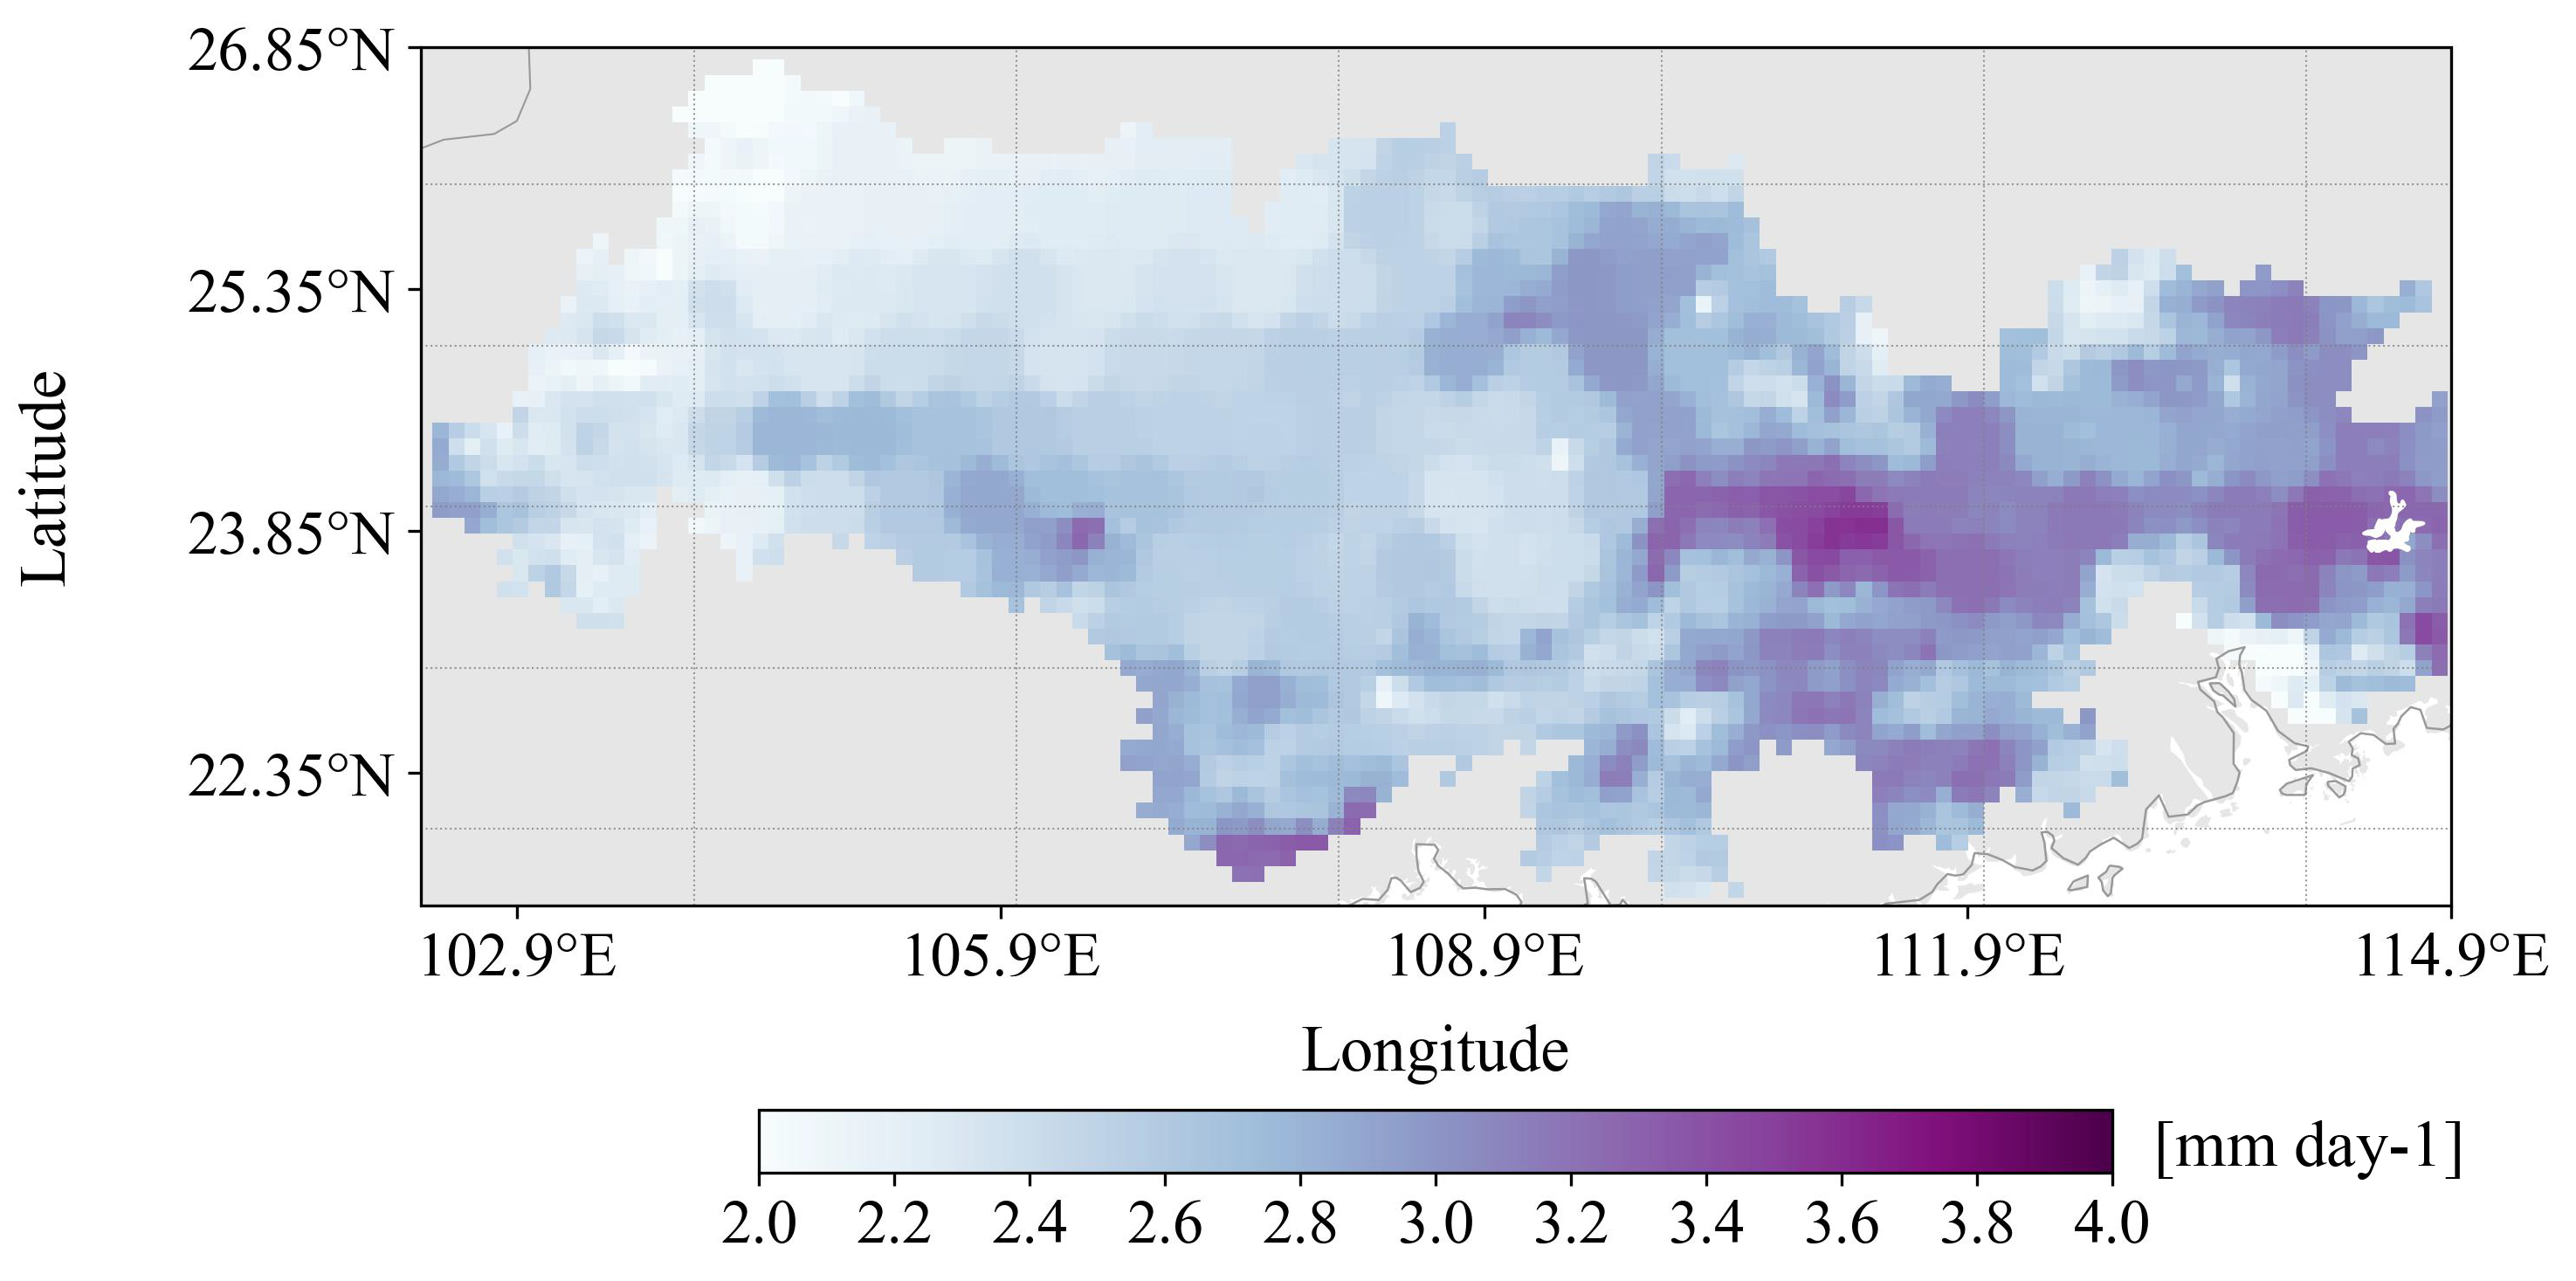
\includegraphics[width=\textwidth]{figures/Example07_PearlRiver_unstr_ET_mean.jpg}
    \caption{珠江流域年平均蒸散发(2001-2010)}
    \label{fig:fig_pearlriver_et}
\end{figure}


图 \ref{fig:fig_pearlriver_et} 展示了案例 7 中 CoLM2024 模拟的珠江流域年平均蒸散发量(2001--2010 年),结果表明该区域蒸散发量介于 2 至 4 mm/day 之间。图 \ref{fig:fig_pearlriver_et_eva} 对比了案例 7 中 CoLM2024 模拟的珠江流域蒸散发量与 GLEAM v4.2a 数据(0.1\textdegree 分辨率,\url{https://www.gleam.eu/\#downloads})。评估表明,基于非结构网格的 CoLM2024 能够准确反映蒸散发的时空变化特征,其蒸散发量预测结果与 GLEAM 数据高度吻合,Adjusted Kling–Gupta efficiency (KGESS)指数多在0.6 以上。

\begin{figure}[htpb]
    \centering
    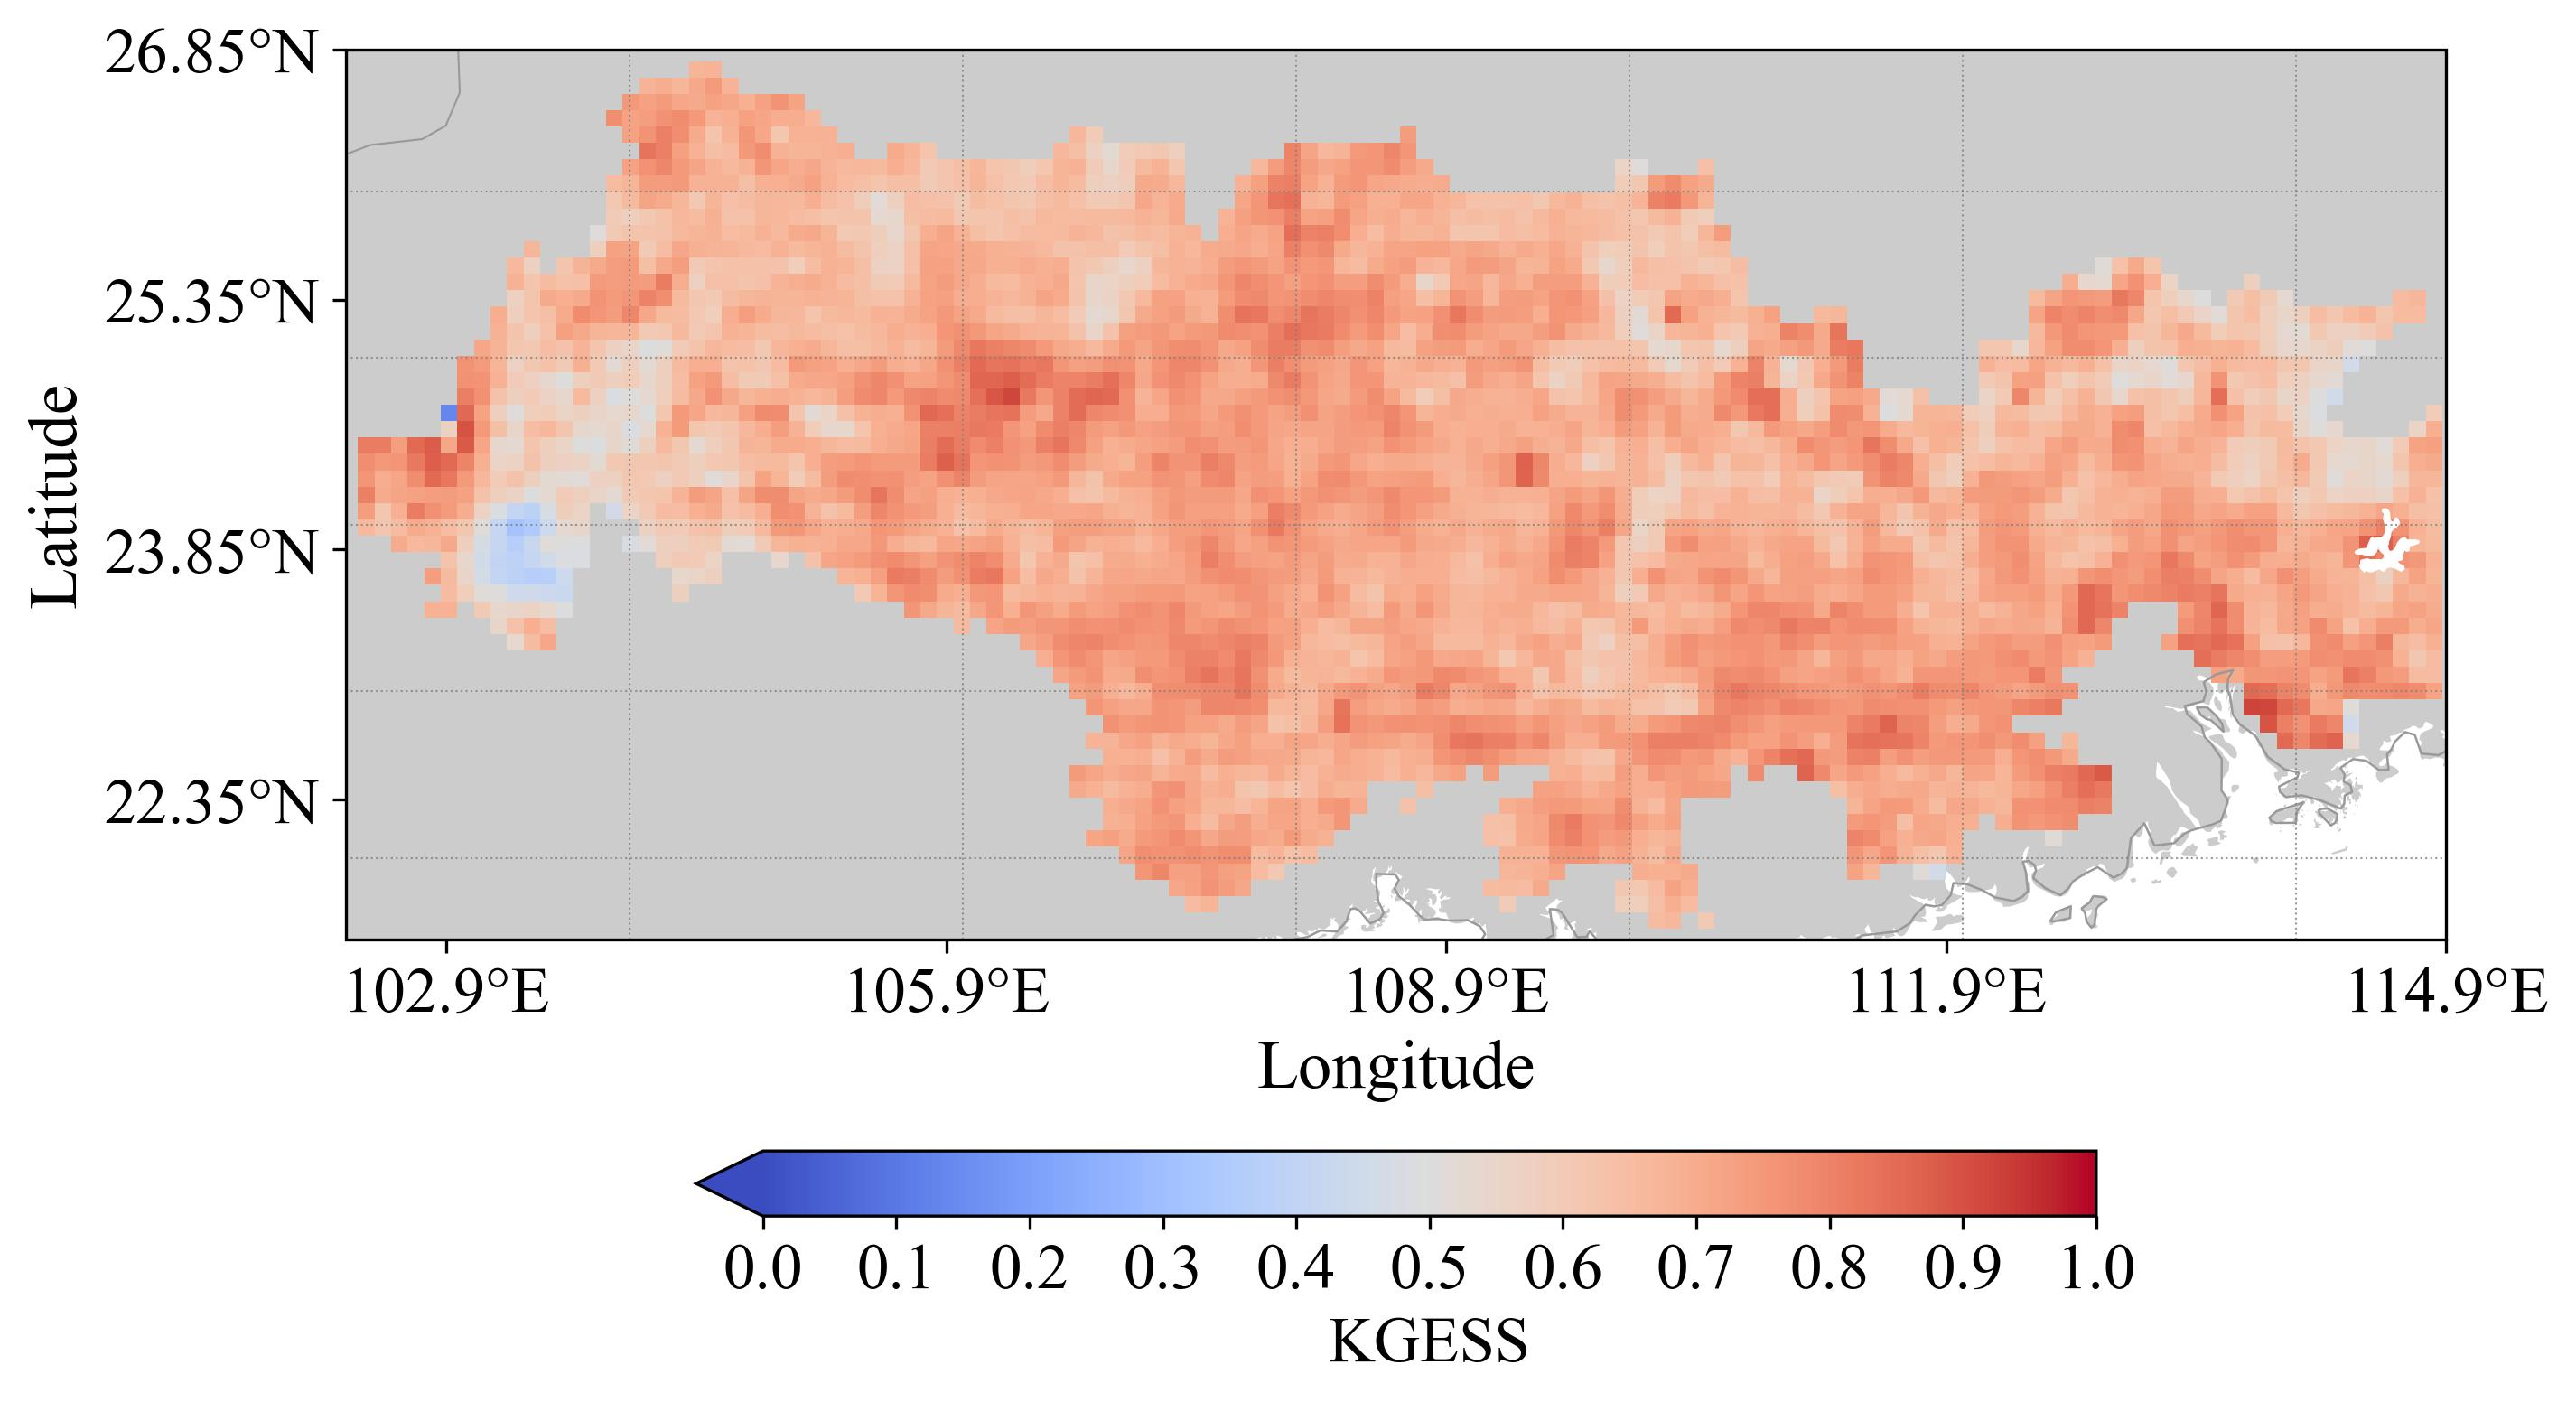
\includegraphics[width=\textwidth]{figures/Example07_PearlRiver_unstr_ET_KGESS.jpg}
    \caption{珠江流域日尺度蒸散发模拟数据与GLEAM参考数据集对比的KGESS分布图}
    \label{fig:fig_pearlriver_et_eva}
\end{figure}


\section{辅助工具包}\label{辅助工具包}
CoLM2024的辅助工具包包括案例创建、案例复制、案例代码比较、创建配置文件、案例代码更新和拷贝代码6个命令组成,这6个命令互相调用,集成不同的功能脚本。create\_newcase和create\_clone是两个案例创建功能脚本,create\_namelist,create\_script、create\_header和copy\_code是四个基础脚本,用于辅助案例的创建。update\_casecode用于版本控制后的案例代码更新。diff\_casecode用于比较两个案例之间,案例和主代码之间的差异。辅助工具包主要是基于案例的概念进行打造的,每个案例拥有独立案例目录,案例目录下包括独立的代码和配置,也就是说对于案例代码的修改,将不会影响其他案例和主代码,这大大地方便模式开发者对于版本的灵活控制。

\subsection{案例目录的结构}
% \subsubsection{案例目录的结构}
执行辅助工具包将自动生成案例目录,案例目录由若干子目录和文件组成,包括代码目录(bld),运行脚本(mksrf.submit, init.submit和case.submit),模拟配置文件(namelist文件),历史文件目录(history$\slash$),重启文件目录(restart$\slash$)和地表数据目录(landdata$\slash$)。其中,代码目录包括源代码目录(bld$\slash$main$\slash$, bld$\slash$mkinidata$\slash$, bld$\slash$mksrfdata$\slash$和bld$\slash$share$\slash$,编译配置文件(bld$\slash$include$\slash$Makeoption)和宏配置文件(bld$\slash$include$\slash$define.h)。历史文件(见章节~\ref{history})、重启文件(见章节~\ref{restart})、地表数据(见章节~\ref{landdata})、namelist文件(见章节~\ref{nml})和宏配置文件(见章节~\ref{define.hux6587ux4ef6})的功能和可选项已在前面章节中详细介绍。代码目录和运行脚本是辅助运行工具包中的新内容。运行脚本用于队列系统的任务提交(如SLURM、LSF和QBS等队列系统),代码目录独立于主目录的代码,可以用于案例的代码修改和初期调试,宏配置文件也在该目录下。修改该目录下的代码或宏文件之后,可以直接编译并单独应用于该案例。

\subsection{辅助工具包的配置}

辅助工具包在移植到新机器使用前需要先编辑机器配置文件和队列系统脚本格式文件,配置并指定数据代码的路径、三个脚本运行需要的核数等机器信息和队列系统脚本格式。机器配置文件包含了新建案例所需的机器信息和数据路径信息(run$\slash$machine.config)见~\ref{table_machineconfig}。

\begin{table}[!htbp]
\caption{机器配置文件变量一览} \label{table_machineconfig}
\centering \renewcommand{\arraystretch}{1.2}
\begin{tabular}{lcp{0.35\textwidth}}
\toprule
\textbf{变量名} & \textbf{示例} & \textbf{说明} \\ \midrule
NProcesses\_mksrf & 672 & mksrf.submit脚本需要的核数 \\
NNodes\_mksrf & 14 & mksrf.submit需要的节点数目 \\
NTasksPerNode\_mksrf & 48 & mksrf.submit单节点核数 \\
Memory\_mksrf & 150G & mksrf.submit运行所申请内存 \\
Walltime\_mksrf & 24:00:00 & mksrf.submit运行所申请时间 \\
Queue\_mksrf & normal & mksrf.submit需要使用的队列 \\
NProcesses\_mkini & 48 &init.submit脚本需要的总核数 \\
NNodes\_mkini & 14 & init.submit需要的节点总数 \\
NTasksPerNode\_mkini & 48 & init.submit单节点核数 \\
Memory\_mkini & 150G & init.submit运行所申请内存 \\
Walltime\_mkini & 24:00:00 & init.submit运行所申请时间 \\
Queue\_mkini & normal & init.submit需要使用的队列 \\
NProcesses\_case & 48 & case.submit脚本需要的核数 \\
NNodes\_case & 14 & case.submit需要的节点数目 \\
NTasksPerNode\_case & 48 & case.submit单节点核数 \\
Memory\_case & 150G & case.submit运行所申请内存 \\
Walltime\_case & 24:00:00 & case.submit运行所申请时间 \\
Queue\_case & normal & case.submit需要使用的队列 \\
Exe\_command & mpirun & 并行提交任务的命令 \\
Exe\_opt & -np & 并行提交任务的选项 \\
BatchSystem & LSF & 队列系统:LSF, PBS, SLURM \\
ROOT & \textasciitilde/CoLM/ & 代码个目录路径 \\
RAWDATA & \textasciitilde/rawdata/ & 模型所需的静态原始数据 \\
RUNTIME & \textasciitilde/runtime/ & 模型所需的动态地表数据 \\
MAKEOPTION & Makeoptions & 编译配置 (模板在include/下) \\
FORCINGPATH & \textasciitilde/CoLM\_Forcing/ &气象驱动数据地址 \\
\bottomrule
\end{tabular}
\end{table}

如需使用队列系统进行任务提交,需要通过编辑队列系统脚本格式文件来配置任务脚本的队列系统头信息格式(run$\slash$batch.config)。

\begin{lstlisting}
##run/batch.config
#------------------------------baiduboat-----------------------------
#!/bin/bash

#BSUB -J <CASENAME>
#BSUB -q <QUEUE>
#BSUB -o colm.o%
#BSUB -e colm.e%
#BSUB -n <NPROCESSES>
#BSUB -R rusage[mem=<MEMORY>]
#BSUB -R span[ptile=<NTASKSPERNODE>]
\end{lstlisting}

其中<CASENAME>是案例名,由案例创建命令create\_newcase收集(章节~\ref{CreateNewcase})。<QUEUE>、<NPROCESSES>、<MEMORY>和<NTASKSPERNODE>分别代表队列名、任务总核数、内存和单节点核数,由机器配置文件(run$\slash$machine.config)收集,见表~\ref{table_machineconfig}。冗余信息需要用\#注释掉。run$\slash$batch.config提供了SLURM、LSF和QBS的模板。

\subsection{案例创建脚本 --- create\_newcase} \label{CreateNewcase}
create\_newcase 将依照用户指定路径创建新的案例,允许用户按照典型案例配置或自定义案例进行配置的方法创建新的案例。其中包括创建namelist文件,创建运行脚本,创建头文件和代码拷贝,它们分别依赖create\_namelist、create\_script、create\_header和copy\_code四个基础脚本来实现。

创建新案例的方法有两种,典型配置创建案例和自定义配置创建案例。两种方法配置案例成功后,依然可以对案例namelist文件和宏定义\texttt{define.h}文件进行修改,手动修改或添加案例配置。

\subsubsection{典型配置创建案例}

典型配置创建案例语法较简单,适合初级用户快速展开模型运行。

语法:

\begin{lstlisting}[xleftmargin=2.5em]
./create_newcase -n {案例运行路径} -c {典型案例配置选项名} [-t {起始年份}] [-e {结束年份}] [-f {气象驱动}]
\end{lstlisting}

案例运行路径为案例的绝对路径或相对路径,要求路径末尾没有"/"符号。典型案例配置选项目前包含5种(见表~\ref{tab:cases_config}),它分别包含了分辨率设置、次网格类型设置、生物地球化学开关和BGC半解析预热开关的设置。


例:
\begin{lstlisting}[xleftmargin=2.5em]
./create_newcase -n ~/CoLM202X/cases/50km_PFT -c Global_Grid_50km_PFT_VG
\end{lstlisting}

\begin{table}[!htbp]
\renewcommand{\arraystretch}{1.5}
\centering
\caption{典型案例配置一览}\label{tab:cases_config}
\begin{tabular}{
cccccc} \toprule
\textbf{典型案例配置选项名} & \textbf{分辨率} & \textbf{次网格} & \textbf{BGC} &\textbf{SASU}\\ \midrule
Global\_Grid\_50km\_PFT\_VG & 0.5\textdegree$\times$0.5\textdegree & PFT & 关 &关\\
Global\_Grid\_50km\_USGS\_VG & 0.5\textdegree$\times$0.5\textdegree & USGS & 关 &关\\
Global\_Grid\_50km\_PC\_VG & 0.5\textdegree$\times$0.5\textdegree & PC & 关 & 关\\
Global\_Grid\_2x2\_PFT\_VG\_BGC & 2.5\textdegree$\times$1.875\textdegree & PFT& 开 &关\\
Global\_Grid\_2x2\_PFT\_VG\_BGC-SASU & 2.5\textdegree$\times$1.875\textdegree & PFT& 开 & 开\\
\bottomrule
\end{tabular}
\end{table}

所有典型案例为全球范围配置,如果未开启生物地球化学循环(BGC)时,默认分辨率为全球50 km,开启BGC时,默认分辨率为全球2.5\textdegree$\times$1.875\textdegree 分辨率。次网格包含植被功能型次网格(PFT),植物群落次网格(PC),地表覆盖类型次网格(LC),其中LC按不同数据来源包含了IGBP和USGS两种。SASU开启时,create\_newcase会自动帮助配置半解析加速预热方案(SASU),SASU仅在生物地球化学循环(BGC)开启时有效。

典型案例设置可以同时通过选项-t和-e设置运行起始和结束年份,通过-f选择气象驱动,通过-i设置预热的类型。时间、驱动和预热选项都是可缺失的,如果没有提供,起始和结束年份的默认值分别是1980年和2000年,气象驱动默认选择CRUJRA,预热选项默认关闭。


\subsubsection{自定义配置创建案例}

自定义配置创建案例通过手动配置模型起始时间、气象驱动、预热类型、格点类型(分辨率)、次网格类型、土壤水力参数模型、河道径流模型CaMa开关、生物地球化学模型开关、作物模型开关。其中,作物模型开关在生物地球化学模型开启时才生效;格点类型(分辨率)、次网格类型、土壤水力参数模型、河道径流模型CaMa开关、生物地球化学模型开关、作物模型开关在没有出现典型配置选项“-c”时才生效。

语法:
\begin{lstlisting}[xleftmargin=2.5em]
./create_newcase -n {案例运行路径} [ -t {开始年份} ] [ -e {结束年份}] [ -f {气象驱动}] [ -g {格点类型} ] [ -s {次网格方案}] [ -m {土壤水力参数模型}] [ -r ] [-b [-p] [-i {预热方案}] ]
\end{lstlisting}

案例运行路径为案例的绝对路径或相对路径,要求路径末尾没有"/"符号。自定义案例配置的详细配置见表~\ref{tab:custom_option}。所有自定义选项均为可缺失选项,缺省值见表~\ref{tab:custom_option}。

例:
\begin{lstlisting}[xleftmargin=2.5em]
./create_newcase -n ~/CoLM202X/cases/50km_PFT -t 1980 -e 2000  -g grid_g144x96 -s PFT -m vg -b -i sasund
\end{lstlisting}

\begin{table}[!htbp]
\renewcommand{\arraystretch}{1.5}
\centering
\caption{自定义案例配置选项一览}\label{tab:custom_option}
\begin{tabular}{
cccccc} \toprule
\textbf{配置选项内容} & \textbf{配置选项} & \textbf{缺省值} & \textbf{备选值} & \textbf{有效条件}\\ \midrule
开始年份 & -t & 1980 & 任意整数 & 始终有效\\
结束年份 & -e & 2000 & 任意整数 & 始终有效\\
气象驱动 & -f & CRUJRA & CRUJRA; GSWP3  & 始终有效\\
格点类型 & -g & $\mathrm{grid}\_\mathrm{g}720\mathrm{x}360$ & 无& 无 -c\\
次网格方案 & -s & PFT & USGS; IGBP; PFT; PC & 无 -c\\
土壤水力模型 & -m & vg & vg; cb& 无 -c\\
Cama模型 & -r & 关 & 无& 无 -c\\
BGC模型 & -b & 关 & 无& 无 -c\\
作物模型 & -p & 关 & 无& 无 -c有 -b\\
预热方案 & -i & none & none; nd; sasund& 无 -c有 -b\\
\bottomrule
\end{tabular}
\end{table}

自定义案例配置选项按照有效条件可以任意组合,对新建案例进行配置,配置完成后,仍然可以通过文本编辑修改\texttt{define.h}, namelist以及三个任务提交脚本进行修改。

\subsection{案例复制脚本 --- create\_clone}

在方案比较实验中,经常需要运行两个配置相似的案例。使用案例复制命令create\_clone可以大大提高工作效率,并且降低配置出错的概率。

语法:
\begin{lstlisting}[xleftmargin=2.5em]
./create_clone -s {待拷贝案例路径} -d {新案例路径}
\end{lstlisting}

例:
\begin{lstlisting}[xleftmargin=2.5em]
./create_clone -s ~/CoLM202X/cases/50km_PFT -d ~/CoLM202X/cases/50km_PFT-new
\end{lstlisting}

待拷贝案例路径和新案例路径都要求路径末尾没有"/"符号。create\_clone语句将拷贝原案例的代码(bld目录)、运行脚本和namelist文件,并且识别案例名,对脚本和namelist中的案例名进行替换。

\subsection{案例的编译和运行}
\subsubsection{案例的编译}
对于案例代码的编译需要进入bld目录,并运行make命令。make前要确认编译配置文件(bld$\slash$include$\slash$Makeoption)的设置是否正确,包括netCDF库,Fortran编译器的选项和路径等(见章节~\ref{comprun})。

\subsubsection{案例目录的运行}
对于典型案例我们提供了适用于队列系统任务提交的三个脚本:地表数据制作任务提交脚本mksrf.submit,初始化任务提交脚本init.submit和模型运行任务提交脚本case.submit,他们分别对应章节~\ref{runcolm}中提到的三个colm运行步骤:地表数据制作、初始场数据制作和主程序运行。运行前需要检查队列系统所需要核数的设置是否和运行mpirun中要求的核数一致,其他内存和队列等配置是否符合服务器的要求。

\subsection{辅助工具包高级功能}

\subsubsection{案例代码的比较 --- diff\_casecode.bash}

在代码开发过程中,需要比较两个代码的差异,案例代码比较脚本可以帮助比较案例代码之间和案例代码与主代码的区别。

语法:

\begin{lstlisting}[xleftmargin=2.5em]
./diff_casecode.bash {待比较案例1路径} [ {待比较案例2路径} ]
\end{lstlisting}

例:
\begin{lstlisting}[xleftmargin=2.5em]
./diff_casecode.bash ~/CoLM202X/cases/50km_PFT ~/CoLM202X/cases/50km_PFT-new1
\end{lstlisting}
或
\begin{lstlisting}[xleftmargin=2.5em]
./diff_casecode.bash  ~/CoLM202X/cases/50km_PFT
\end{lstlisting}

diff\_casecode.bash后可接两个参数或一个参数,参数指明案例路径,要求路径末尾没有``/"符号。当脚本命令后接两个参数并指定两个案例路径时,脚本将比较两个案例代码之间每行的差异。当脚本命令后接一个参数并制定一个案例路径时,脚本将比较该案例代码和主代码之间的差异,主代码路径需要通过编辑diff\_casecode.bash文件``ROOT="行内容来指定。

\subsubsection{案例namelist文件的创建 --- create\_namelist}

模式运行的namelist文件可以通过create\_namelist脚本来创建。create\_namelist根据输入的开始结束年份、气象驱动、原始地表数据路径、运行数据路径、陆海分布数据、BGC预热方案和运行区域信息写入namelist文件。create\_namelist脚本所有选项一览表见表~\ref{tab:createnml_option}。

语法:
\begin{lstlisting}[xleftmargin=2.5em]
./create_namelist {案例路径} {案例名} [-t {开始年份} ] [ -e {结束年份}] [ -f {气象驱动}] [ -d {原始地表数据路径}] [ -r {运行时数据路径}] [ -a {格点纬向分辨率} ] [ -o {格点经向分辨率} ] [ -S {区域南边界纬度} ] [ -N {区域北边界纬度} ] [ -E {区域东边界经度} ] [ -W {区域西边界经度} ] [ -i {BGC预热方案} ] [ -x {经向数据分块数目}] [ -y {纬向数据分块数目}][-g {每 IO 组的进程数量}]
\end{lstlisting}

例:
\begin{lstlisting}[xleftmargin=2.5em]
./create_namelist -p ~/CoLM202X/cases/ -n 50km_PFT -a 0.5 -o 0.5
\end{lstlisting}

\begin{table}[!htbp]
\renewcommand{\arraystretch}{1.5}
\centering
\caption{create\_namelist配置选项一览}\label{tab:createnml_option}
\begin{tabular}{
cccccc} \toprule
\textbf{配置选项内容} & \textbf{配置选项} & \textbf{缺省值} & \textbf{备选值} & \textbf{有效条件}\\ \midrule
案例路径 & -p & 不可缺省 & 任意路径 & 始终有效 \\
案例名  & -n & 不可缺省 & 任意字符串 & 始终有效 \\
开始年份 & -t & 1980 & 任意整数 & 始终有效\\
结束年份 & -e & 2000 & 任意整数 & 始终有效\\
气象驱动 & -f & CRUJRA & CRUJRA; GSWP3  & 始终有效\\
原始地表数据路径 & -d & 无 & 任意路径 & 始终有效\\
运行数据路径 & -r & 无 & 任意路径 & 始终有效\\
经向分辨率 & -a & 0.5 & 任意数值 & 始终有效\\
纬向分辨率 & -o & 0.5 & 任意数值 & 始终有效\\
海陆分布数据路径 & -l & 无 & 任意路径 & 始终有效\\
区域南边界纬度 & -S & -90 & -90.0\textasciitilde90.0 小于北边界纬度 & 始终有效\\
区域北边界纬度 & -N & 90 & -90.0\textasciitilde90.0 大于南边界纬度 & 始终有效\\
区域西边界经度 & -S & -180 & -180.0\textasciitilde180.0 小于东边界经度 & 始终有效\\
区域东边界经度 & -N & 180 & -180.0\textasciitilde180.0 大于西边界经度 & 始终有效\\
BGC预热开关 & -i &none & none; nd; sasund& 始终有效 \\
经向数据分块数目 & -x & 18 & 大于1的整数& 始终有效 \\
纬向数据分块数目 & -y & 9 & 大于1的整数& 始终有效 \\
每IO组的进程数量 & -g & 24 & 大于1的整数& 始终有效 \\
\bottomrule
\end{tabular}
\end{table}

\subsubsection{案例脚本的创建 --- create\_script}

create\_script可以帮助用户生成可用于队列系统的三个任务脚本,1)地表数据制作程序提交脚本mksrf.submit; 2)冷启动程序提交脚本init.submit;3)CoLM程序提交脚本case.submit。每个任务脚本根据batch.config和machine.config的内容来完成头信息的配置,它指定节点数目、CPU数目、内存使用和运行时间长度。create\_script脚本所有选项一览表见表~\ref{tab:createscript_option}。

create\_script根据BGC预热开关的设置(-i选项),为case.submit配置三种不同的预热方式:1) none, 2) nd, 3) sausund。BGC预热要求用脚本来控制单年驱动循环,1) none方式不包含BGC预热,可以用于非循环的模拟,为默认方案;2) nd方式为一年驱动循环的预热方式,case.submit中包含循环末尾对重启文件的重命名(时间戳的重命名),默认完成100次循环,可生脚本后通过手动编辑case.submit进行修改。3) sasund方式同为1年驱动循环的预热,case.submit中包含循环末尾对重启文件的重命名(时间戳重命名),默认完成130次循环,但前100次为半解析加速预热,后三十次为普通预热方式,类同于nd方式。

语法
\begin{lstlisting}[xleftmargin=2.5em]
./create_scripts -p {案例路径} -t {开始年份} -e {结束年份} -f {batch配置文件路径} -c {机器配置文件路径} -i {BGC预热方案}
\end{lstlisting}

例:
\begin{lstlisting}[xleftmargin=2.5em]
./create_scripts -p ~/CoLM202X/cases/50km_PFT -t 1850 -e 1850 -f ~/CoLM202X/run/batch.config -c ~/CoLM202X/run/machine.config -i nd
\end{lstlisting}

\begin{table}[!htbp]
\renewcommand{\arraystretch}{1.5}
\centering
\caption{create\_script配置选项一览}\label{tab:createscript_option}
\begin{tabular}{
cccccc} \toprule
\textbf{配置选项内容} & \textbf{配置选项} & \textbf{缺省值} & \textbf{备选值} & \textbf{有效条件}\\ \midrule
案例路径名 & -p & 不可缺省 & 任意路径 & 始终有效 \\
开始年份 & -t & 不可缺省 & 任意整数 & 始终有效\\
结束年份 & -e & 不可缺省 & 任意整数 & 始终有效\\
batch配置文件路径 & -f & 不可缺省 & 任意路径 & 始终有效 \\
机器配置文件路径 & -f & 不可缺省 & 任意路径 & 始终有效 \\
BGC预热开关 & -i &none & none; nd; sasund& 始终有效 \\
\bottomrule
\end{tabular}
\end{table}

\subsubsection{案例代码更新 --- update\_casecode}

随着代码的发展,本地仓库会通过github进行更新。案例代码常常需要随着本地仓库代码的更新而更新。运用案例代码更新脚本可以帮助实现案例代码的更新。但需注意,案例代码更新脚本仅仅实现拷贝覆盖代码的功能,尚无法实现代码合并(merge)的功能。因此,更新代码前须妥善处理案例代码已更新的部分。注意:在使用前,需要编辑update\_casecode中的ROOT变量,定位本地仓库代码。

语法:
\begin{lstlisting}[xleftmargin=2.5em]
./update_casecode {待更新的案例路径}
\end{lstlisting}
另外,确保待更新的案例路径后没有"/"。

例:
\begin{lstlisting}[xleftmargin=2.5em]
./update_casecode ~/CoLM202X/cases/50km_PFT
\end{lstlisting}

\subsubsection{案例代码更新 --- diffcasecode.bash}

diffcasecode.bash将比较两个案例代码之间的差异,或者比较单一案例代码和本地仓库代码的差异,差异显示将精确到每个文件的每一行。运用该脚本可以帮助代码开发者在更新本地仓库前,看清代码的改动,并进一步清理更新本地仓库代码。

语法:

\begin{lstlisting}[xleftmargin=2.5em]
./diffcasecode.bash {待比较案例1路径} [{待比较案例2路径}]
\end{lstlisting}

当脚本存在两个参数时,脚本将比较两个案例之间的代码差异,当脚本仅存在一个参数时,代码将比较指定案例代码和本地仓库代码的差异。

例:
\begin{lstlisting}[xleftmargin=2.5em]
./diffcasecode.bash ~/CoLM202X/cases/50km_PFT1/
\end{lstlisting}
或
\begin{lstlisting}[xleftmargin=2.5em]
./diffcasecode.bash ~/CoLM202X/cases/50km_PFT1/ ~/CoLM202X/cases/50km_PFT2
\end{lstlisting}

第一个例子比较50km\_PFT1案例和本地仓库代码的差异,第二个例子比较案例50km\_PFT1和案例50km\_PFT2代码之间的差异。


\subsubsection{案例代码复制 --- copy\_code}
copy\_code将原案例或本地仓库代码拷贝到新案例代码路径,是案例复制脚本(create\_clone)和案例代码更新脚本(update\_casecode)的一部分。相比create\_clone,copy\_code的差异在于它仅拷贝代码不操作namelist和任务脚本文件。注意:案例代码路径需要给到案例的bld目录地址,本地仓库代码路径给到本地仓库地址即可。

语法:
\begin{lstlisting}[xleftmargin=2.5em]
./copy_code -s {待复制代码路径} -d {目标代码路径}
\end{lstlisting}

例:
\begin{lstlisting}[xleftmargin=2.5em]
./copy_code -s ~/CoLM202X/cases/50km_PFT/bld -d ~/CoLM202X/cases/50km_PFT-new1/bld
\end{lstlisting}
或
\begin{lstlisting}[xleftmargin=2.5em]
./copy_code -s ~/CoLM202X -d ~/CoLM202X/cases/50km_PFT-new1/bld
\end{lstlisting}
第二个例子等同于用update\_casecode更新案例50km\_PFT-new1

\subsubsection{重启数据的复制 --- copy\_restart}
copy\_restart通过拷贝现成的重启数据来帮助用户热启动新案例。CoLM的案例热启动需要重启数据,CoLM通过重启数据的案例名、日期和时间来识别案例的重启数据文件。因此,直接拷贝现成案例的重启数据,并无法被新案例识别。因此,copy\_restart脚本通过拷贝和重命名重启数据文件名来让已有重启数据匹配新案例所能识别的文件名。

语法:
\begin{lstlisting}[xleftmargin=2.5em]
./copy_restart -s {待复制重启文件所属案例路径} -d {目标案例路径} -o {待复制重启数据的时间点} [ -e {目标案例重启时间点}]
\end{lstlisting}

前面三个参数是必须提供的,第四个参数"-e"为可缺省参数,不提供时,脚本将把原案例同时间点的重启文件复制到目标案例中,当“-e”参数提供时,脚本将把目标案例的重启时间点修改为指定的时间点。同时,用户需要确认指定的时间点是否与Namelist文件中的起始时间一致,否则CoLM依然无法找到正确的重启文件。
%\clearpage
